\documentclass[a4paper,12pt]{article}
\usepackage[left=2cm,right=2cm,top=2.5cm,bottom=2.5cm]{geometry}
\usepackage{amsmath,amssymb,graphicx,booktabs,array,float}
\usepackage{algorithm,algpseudocode}
\usepackage{caption}
\captionsetup[table]{position=top,labelfont=bf,labelsep=newline,justification=raggedright,singlelinecheck=false,skip=5pt}
\usepackage[colorlinks=true,linkcolor=blue,citecolor=blue,urlcolor=blue]{hyperref}
\setlength{\parindent}{0pt}
\setlength{\parskip}{0.5em}
\setlength{\emergencystretch}{1.5em}
\newcommand{\vect}[1]{\boldsymbol{#1}}
\newcommand{\matr}[1]{\boldsymbol{#1}}
\algrenewcommand\algorithmicrequire{\textbf{Input:}}
\algrenewcommand\algorithmicensure{\textbf{Output:}}
\title{Notes on by-mode ECSW for LSPG reduced-order models}
\author{}
\date{October 5, 2026}
\newcommand{\FOMMeanMinutes}{5.404}
\newcommand{\ECSWFOMSpeedup}{17.39}
\newcommand{\BMFOMSpeedup}{267.93}
\newcommand{\ECSWMinSeconds}{18.54}
\newcommand{\ECSWMaxSeconds}{18.83}
\newcommand{\BMMinSeconds}{1.20}
\newcommand{\BMMaxSeconds}{1.22}
\newcommand{\ECSWMaxGlobalError}{1.0959}
\newcommand{\BMMaxGlobalError}{1.1019}
\newcommand{\BMLargestErrorIncrease}{0.0141}
\newcommand{\BMMinIterationsTotal}{1\,509}
\newcommand{\BMMaxIterationsTotal}{1\,518}
\newcommand{\BMConvergedSteps}{4\,500}

\newcommand{\ECSWOfflineMinutes}{112.56}
\newcommand{\BMOfflineMinutes}{4.10}
\newcommand{\OfflineTrainingRatio}{27.48}

\begin{document}
\maketitle

BM-ECSW was proposed by Sebastian Rodriguez~\cite{rodriguez2026proposal}. Its mode-dependent cubature weights are applied here to LSPG reduced-order models.

\section{Projection-based reduced-order models}
\label{sec:prom}

The construction of a projection-based reduced-order model (PROM) begins by collecting $N_s$ solution snapshots $\vect{u}_s\in\mathbb R^N$ of a high-dimensional model (HDM), where $N$ denotes the number of degrees of freedom of the original model. These snapshots sample the evolution of the solution at selected times and parameter values. Given a fixed reference state $\vect{u}_{\mathrm{ref}}$, their deviations from this state are assembled into a snapshot matrix and compressed using a thin singular value decomposition (SVD):
\begin{equation}
 \begin{aligned}
 \matr{S}
 &=[\vect{u}_1-\vect{u}_{\mathrm{ref}},\ldots,
     \vect{u}_{N_s}-\vect{u}_{\mathrm{ref}}]
     \in\mathbb R^{N\times N_s},\\
 \matr{S}&=\matr{U}_S\matr{\Sigma}_S\matr{Y}_S^T.
 \end{aligned}
 \label{eq:pod-snapshots}
\end{equation}
Here $\matr{U}_S$ and $\matr{Y}_S$ contain the left and right singular vectors, respectively, and $\matr{\Sigma}_S$ contains the singular values $\sigma_{S,i}$ in descending order. The proper orthogonal decomposition (POD) basis is formed by retaining the first $n\ll N$ left singular vectors, yielding the orthonormal reduced-order basis (ROB)
\begin{equation}
 \matr{V}=\matr{U}_S(:,1:n)
         =[\vect{v}_1,\ldots,\vect{v}_n]
         \in\mathbb R^{N\times n},
 \qquad \matr{V}^T\matr{V}=\matr{I}_n.
 \label{eq:pod-basis}
\end{equation}
The reduced dimension $n$ is selected using the singular value energy truncation criterion
\begin{equation}
 1-\frac{\displaystyle\sum_{i=1}^{n}\sigma_{S,i}^2}
         {\displaystyle\sum_{j=1}^{\min(N,N_s)}\sigma_{S,j}^2}
 \leq\varepsilon_S^2,
 \label{eq:pod-tolerance}
\end{equation}
where $\varepsilon_S>0$ controls the discarded fraction of the sum of squared singular values.

Using the ROB in Equation~\eqref{eq:pod-basis}, the HDM state is approximated as
\begin{equation}
 \widetilde{\vect{u}}(\vect{q})
 =\vect{u}_{\mathrm{ref}}+\matr{V}\vect{q}
 =\vect{u}_{\mathrm{ref}}+\sum_{i=1}^nq_i\vect{v}_i.
 \label{eq:affine}
\end{equation}
In this approximation, the columns $\vect{v}_i$ of $\matr{V}$ are the POD modes, and $\vect{q}\in\mathbb R^n$ is the vector of generalized coordinates. The reference state and ROB remain fixed, while the coordinates depend on time and parameters. Equation~\eqref{eq:affine} therefore restricts the approximate state to an $n$-dimensional affine trial space. The evolution of its coordinates is determined by projecting the governing equations onto a suitable test space.

\subsection{Least-squares Petrov--Galerkin projection}
\label{sec:lspg}

Consider a parametric, nonlinear, semi-discrete first-order initial-value problem of the form
\begin{equation}
 \matr{M}(\vect{\mu})\dot{\vect{u}}(t;\vect{\mu})
 +\vect{f}(\vect{u}(t;\vect{\mu});\vect{\mu})
 -\vect{g}(t;\vect{\mu})=\vect{0},
 \qquad \vect{u}(0;\vect{\mu})=\vect{u}_0(\vect{\mu}).
 \label{eq:hdm}
\end{equation}
Here $\vect{u}(t;\vect{\mu})\in\mathbb R^N$ is the HDM state, $\matr{M}$ is the mass matrix, $\vect{f}$ contains the internal or flux terms, and $\vect{g}$ contains the forcing terms. The vector $\vect{\mu}\in\mathcal D$ specifies the parameters, and a dot denotes differentiation with respect to time. Applying an implicit time discretization to Equation~\eqref{eq:hdm} gives the nonlinear system
\begin{equation}
 \vect{r}^{m+1}(\vect{u}^{m+1};\vect{\mu})=\vect{0},
 \label{eq:discrete-hdm}
\end{equation}
where $\vect{r}^{m+1}\in\mathbb R^N$ is the time-discrete HDM residual and the superscript $m+1$ identifies the time level $t^{m+1}$. The parameters and all history states required by the time integrator are held fixed during the solution at this time level; the history states are omitted from the residual arguments.

Substituting the affine approximation in Equation~\eqref{eq:affine} into Equation~\eqref{eq:discrete-hdm} yields $N$ equations for the $n$ generalized coordinates. This system is generally overdetermined. Least-squares Petrov--Galerkin (LSPG) projection determines the coordinates by minimizing the Euclidean norm of the time-discrete residual~\cite{carlberg2011efficient,ares2026closure}:
\begin{equation}
 \vect{q}^{m+1}\in\underset{\vect{q}\in\mathbb R^n}{\arg\min}\;
 \Phi(\vect{q}),\qquad
 \Phi(\vect{q})=\frac12\left\|\vect{r}^{m+1}
     (\vect{u}_{\mathrm{ref}}+\matr{V}\vect{q})\right\|_2^2.
 \label{eq:lspg-objective}
\end{equation}
The residual in this objective is evaluated with the known approximate history states and the prescribed parameters, which are omitted from its arguments. To express the stationarity conditions of Equation~\eqref{eq:lspg-objective}, define the HDM residual Jacobian and the LSPG test basis as
\begin{equation}
 \begin{aligned}
 \matr{J}(\widetilde{\vect{u}})
 &=\frac{\partial\vect{r}^{m+1}}{\partial\widetilde{\vect{u}}}
 \in\mathbb R^{N\times N},\\
 \matr{W}(\vect{q})
 &=\frac{\partial\vect{r}^{m+1}(\widetilde{\vect{u}}(\vect{q}))}{\partial\vect{q}}
 =\matr{J}(\widetilde{\vect{u}}(\vect{q}))\matr{V}
 \in\mathbb R^{N\times n}.
 \end{aligned}
 \label{eq:test-basis}
\end{equation}
The last equality follows from the chain rule and the fixed affine approximation, for which $\partial\widetilde{\vect{u}}/\partial\vect{q}=\matr{V}$. Thus the test basis depends on the current state through the HDM residual Jacobian. Differentiating the least-squares objective using Equation~\eqref{eq:test-basis} gives the projected residual and the resulting stationarity equations:
\begin{equation}
 \begin{aligned}
 \vect{r}_n(\vect{q})
 &=\nabla_{\vect{q}}\Phi(\vect{q})
 =\matr{W}(\vect{q})^T\vect{r}^{m+1}(\widetilde{\vect{u}}(\vect{q})),\\
 \vect{r}_n(\vect{q}^{m+1})&=\vect{0}.
 \end{aligned}
 \label{eq:projected-residual}
\end{equation}
These $n$ nonlinear equations express the orthogonality of the discrete HDM residual to the test space spanned by the columns of $\matr{W}$ and determine the generalized coordinates at the new time level.

The nonlinear least-squares problem in Equation~\eqref{eq:lspg-objective} is solved using a Gauss--Newton iteration~\cite{carlberg2013gnat}. At iteration $k$ within time step $m+1$, let $\matr{W}^{m+1,k}=\matr{W}(\vect{q}^{m+1,k})$. Linearizing the residual with respect to a coordinate increment $\Delta\vect{q}$ around the current iterate gives
\begin{equation}
 \vect{r}^{m+1}\!\left(\widetilde{\vect{u}}(\vect{q}^{m+1,k}+\Delta\vect{q})\right)
 \approx\vect{r}^{m+1}\!\left(\widetilde{\vect{u}}(\vect{q}^{m+1,k})\right)
       +\matr{W}^{m+1,k}\Delta\vect{q}.
\end{equation}
The Gauss--Newton correction minimizes the Euclidean norm of this linearized residual. Its normal equations are
\begin{equation}
 \left(\matr{W}^{m+1,k}\right)^T\matr{W}^{m+1,k}
       \Delta\vect{q}^{m+1,k+1}
 =-\left(\matr{W}^{m+1,k}\right)^T
       \vect{r}^{m+1}\!\left(\widetilde{\vect{u}}(\vect{q}^{m+1,k})\right),
 \label{eq:gn}
\end{equation}
with all quantities evaluated at the current iterate. Solving this $n\times n$ system gives the coordinate correction used in the update
\begin{equation}
 \vect{q}^{m+1,k+1}
 =\vect{q}^{m+1,k}+\Delta\vect{q}^{m+1,k+1}.
\end{equation}
The residual and test basis are then evaluated at the updated state to form the next correction. This procedure is repeated until the projected equations in Equation~\eqref{eq:projected-residual} satisfy the prescribed nonlinear convergence criterion.


\section{Classical energy-conserving sampling and weighting (ECSW)}
\label{sec:ecsw}
\label{sec:meshes}

Although LSPG projection reduces the number of unknowns from $N$ to $n\ll N$, assembling the reduced equations still requires evaluating the HDM residual and the LSPG test basis on the original mesh. For nonlinear PROMs, these quantities depend on the current reduced state and are evaluated at each Gauss--Newton iteration to form the system in Equation~\eqref{eq:gn}. The computational cost of this assembly therefore remains dependent on the HDM dimension $N$, which can limit the acceleration achieved in applications requiring repeated or rapid predictions. Hyperreduction addresses this dependence by evaluating only a subset of the contributions needed to assemble the reduced equations. The energy-conserving sampling and weighting (ECSW) method~\cite{farhat2014dimensional,farhat2015structure,chapman2017accelerated,grimberg2021mesh} constructs such an approximation using positive cubature weights on a sampled mesh. Originally developed for nonlinear structural dynamics, the method has been extended to Petrov--Galerkin PROMs of first-order dynamical systems.

To construct this approximation, consider the set of mesh entities $\mathcal E=\{e_1,\ldots,e_{N_e}\}$ associated with the HDM discretization. An entity can be a node or a cell, depending on the spatial discretization. Each entity $e$ is associated with a block of $d_e$ assembled residual entries, and these blocks form a nonoverlapping partition of the global residual. The Boolean matrix $\matr{L}_e\in\{0,1\}^{d_e\times N}$ selects the residual rows belonging to this block, while $\matr{L}_{e^+}\in\{0,1\}^{d_e^+\times N}$ selects the state entries required to evaluate it, including those of neighboring entities within the numerical stencil. The residual partition satisfies
\begin{equation}
 \sum_{e\in\mathcal E}\matr{L}_e^T\matr{L}_e=\matr{I}_N.
 \label{eq:residual-partition}
\end{equation}
This partition is applied to assembled residual rows; element contributions that share degrees of freedom are combined before forming these blocks. At a fixed time level, the residual block of entity $e$ can be written as
\begin{equation}
 \vect{r}_e(\vect{q})
 =\matr{L}_e\vect{r}^{m+1}(\widetilde{\vect{u}}(\vect{q}))
 =\vect{r}_e^{m+1}\!\left(
    \matr{L}_{e^+}(\vect{u}_{\mathrm{ref}}+\matr{V}\vect{q})\right)
 \in\mathbb R^{d_e},
 \label{eq:entity-blocks}
\end{equation}
where the prescribed parameters and known history states are held fixed and omitted from the arguments. Embedding these local blocks into the global residual space gives
\begin{equation}
 \vect{r}^{m+1}(\widetilde{\vect{u}}(\vect{q}))
 =\sum_{e\in\mathcal E}\matr{L}_e^T\vect{r}_e(\vect{q}).
 \label{eq:residual-assembly}
\end{equation}
Substituting this assembly into Equation~\eqref{eq:projected-residual} expresses the LSPG projected residual as a sum over the original mesh:
\begin{equation}
 \begin{aligned}
 \vect{r}_n(\vect{q})
 &=\matr{W}(\vect{q})^T
       \vect{r}^{m+1}(\widetilde{\vect{u}}(\vect{q}))\\
 &=\sum_{e\in\mathcal E}
       \matr{W}(\vect{q})^T\matr{L}_e^T\vect{r}_e(\vect{q}).
 \end{aligned}
 \label{eq:full-projected-sum}
\end{equation}
The contribution of each entity is obtained by restricting the test basis to its residual rows. Defining
\begin{equation}
 \matr{W}_e=\matr{L}_e\matr{W}
           =\frac{\partial\vect{r}_e}{\partial\vect{q}},
 \qquad
 \vect{g}_e=\matr{W}_e^T\vect{r}_e,
 \qquad
 \vect{r}_n=\sum_{e\in\mathcal E}\vect{g}_e,
 \label{eq:entity-contribution}
\end{equation}
gives $\matr{W}_e\in\mathbb R^{d_e\times n}$ and $\vect{g}_e\in\mathbb R^n$. Thus each local residual block supplies a contribution to all $n$ reduced equations.

ECSW approximates the full projected sum in Equation~\eqref{eq:full-projected-sum} using a sampled subset $\widetilde{\mathcal E}\subset\mathcal E$, with $n_e=|\widetilde{\mathcal E}|\ll N_e$, and one positive scalar weight $\xi_e$ per selected entity:
\begin{equation}
 \begin{aligned}
 \vect{r}_n(\vect{q})
 &\approx\widetilde{\vect{r}}_n^{\mathrm{ECSW}}(\vect{q})\\
 &=\sum_{e\in\widetilde{\mathcal E}}
      \xi_e\matr{W}(\vect{q})^T\matr{L}_e^T\vect{r}_e(\vect{q})
 =\sum_{e\in\widetilde{\mathcal E}}\xi_e\vect{g}_e(\vect{q}).
 \end{aligned}
 \label{eq:classical}
\end{equation}
The weight $\xi_e$ multiplies every component of $\vect{g}_e$, so it is shared by all reduced equations. The sampled mesh and these weights are trained together so that the weighted contributions approximate the full projected residual over a set of training configurations to within a prescribed tolerance~\cite{grimberg2021mesh}. Once this cubature rule is fixed, the generalized coordinates are obtained at each time step by setting the approximated projected residual to zero.

Evaluating the sampled sum in Equation~\eqref{eq:classical} requires the state entries selected by $\matr{L}_{e^+}$ for every $e\in\widetilde{\mathcal E}$. These dependencies can extend beyond the sampled entities. The union of the sampled mesh and its required stencil neighbors defines the augmented mesh $\widetilde{\mathcal E}^{+}$, with
\begin{equation}
 n_e=|\widetilde{\mathcal E}|,\qquad
 n_e^+=|\widetilde{\mathcal E}^{+}|,\qquad n_e\leq n_e^+\leq N_e.
 \label{eq:mesh-sizes}
\end{equation}
Both sizes count mesh entities. Let $\mathcal I^+$ denote the scalar state indices belonging to $\widetilde{\mathcal E}^{+}$. Restricting the reference state and the ROB to these indices gives
\begin{equation}
 \vect{u}_{\mathrm{ref}}^+=\vect{u}_{\mathrm{ref}}(\mathcal I^+),\qquad
 \matr{V}^+=\matr{V}(\mathcal I^+,:).
 \label{eq:augmented-basis}
\end{equation}
The affine approximation can then be evaluated on the augmented mesh as
\begin{equation}
 \widetilde{\vect{u}}^+(\vect{q})
 =\vect{u}_{\mathrm{ref}}^++\matr{V}^+\vect{q}
 \in\mathbb R^{|\mathcal I^+|}.
 \label{eq:augmented-affine}
\end{equation}
Using this restricted state to evaluate the selected residual blocks, the corresponding test-basis blocks follow from the chain rule:
\begin{equation}
 \matr{W}_e(\vect{q})
 =\frac{\partial\vect{r}_e}{\partial\widetilde{\vect{u}}^+}
    \matr{V}^+,
 \qquad e\in\widetilde{\mathcal E}.
 \label{eq:local-test-basis}
\end{equation}
Here the local residual derivative has dimensions $d_e\times|\mathcal I^+|$ and $\matr{V}^+$ has dimensions $|\mathcal I^+|\times n$. Consequently, the state reconstruction and local evaluations needed during the online iterations depend on the reduced dimension and the sizes of the sampled and augmented meshes.

\subsection{Offline mesh sampling and weight fitting}

The cubature rule in Equation~\eqref{eq:classical} is constructed from $N_c$ training configurations, each comprising a trial state, its parameters, and the known history required by the time-discrete residual. These states can be obtained from the HDM solution snapshots by orthogonal projection onto the affine trial space:
\begin{equation}
 \overline{\vect{u}}
 =\vect{u}_{\mathrm{ref}}+\matr{V}\matr{V}^T
    (\vect{u}_{\mathrm{HDM}}-\vect{u}_{\mathrm{ref}}).
 \label{eq:projection}
\end{equation}
When the residual depends on history states, the same projection is applied to those snapshots. Evaluating the local residuals and test-basis blocks at each configuration $c=1,\ldots,N_c$ gives the projected entity contributions and their full sum:
\begin{equation}
 \vect{g}_e^{(c)}=(\matr{W}_e^{(c)})^T\vect{r}_e^{(c)}\in\mathbb R^n,
 \qquad
 \vect{b}^{(c)}=\sum_{e\in\mathcal E}\vect{g}_e^{(c)}.
 \label{eq:sampled-training-contribution}
\end{equation}
Stacking these contributions over the training configurations produces the matrix and target vector
\begin{equation}
 \matr{G}=
 \begin{bmatrix}
   \vect{g}_{e_1}^{(1)}&\cdots&\vect{g}_{e_{N_e}}^{(1)}\\
   \vdots&\ddots&\vdots\\
   \vect{g}_{e_1}^{(N_c)}&\cdots&\vect{g}_{e_{N_e}}^{(N_c)}
 \end{bmatrix}
 =[\vect{g}_1,\ldots,\vect{g}_{N_e}],
 \qquad
 \vect{b}=
 \begin{bmatrix}
   \vect{b}^{(1)}\\ \vdots\\ \vect{b}^{(N_c)}
 \end{bmatrix}.
 \label{eq:training-matrix}
\end{equation}
Here $\matr{G}\in\mathbb R^{nN_c\times N_e}$ and $\vect{b}\in\mathbb R^{nN_c}$. Column $\vect{g}_e$ contains the contributions of one entity across all configurations, and each configuration supplies $n$ rows. In particular, $G_{(c-1)n+i,e}=g_{e,i}^{(c)}$. Since the target is the sum of all entity contributions, these quantities satisfy
\begin{equation}
 \matr{G}\vect{1}=\vect{b},
 \label{eq:training-assembly}
\end{equation}
where $\vect{1}\in\mathbb R^{N_e}$ is the vector of ones.

The training task is therefore to replace the full sum by a sparse, nonnegative weight vector whose weighted contributions reproduce $\vect{b}$ to the required accuracy. This leads to the ideal sampling problem
\begin{equation}
 \underset{\vect{\xi}\in\mathbb R^{N_e},\ \vect{\xi}\geq\vect{0}}
            {\min}\ \|\vect{\xi}\|_0
 \quad\text{subject to}\quad
 \|\matr{G}\vect{\xi}-\vect{b}\|_2\leq\tau\|\vect{b}\|_2,
 \qquad 0<\tau<1,
 \label{eq:classical-sparse-problem}
\end{equation}
where $\|\vect{\xi}\|_0$ counts the nonzero weights and $\tau$ is the prescribed relative training tolerance. Each entry of $\vect{\xi}$ corresponds to one original mesh entity, and its positive support defines the reduced mesh:
\begin{equation}
 \widetilde{\mathcal E}=\{e\in\mathcal E:\xi_e>0\},
 \qquad n_e=|\widetilde{\mathcal E}|.
 \label{eq:classical-support}
\end{equation}
Because the cardinality problem in Equation~\eqref{eq:classical-sparse-problem} is combinatorial, the sampled set is constructed progressively using nonnegative least-squares (NNLS) fits~\cite{chapman2017accelerated}. The fitting objective is
\begin{equation}
 \underset{\vect{\xi}\geq\vect{0}}{\min}\;
 F(\vect{\xi}),\qquad
 F(\vect{\xi})=\frac12\|\matr{G}\vect{\xi}-\vect{b}\|_2^2.
 \label{eq:classical-nnls-global}
\end{equation}
The NNLS fits determine the weights on the selected entities, while progressive selection and stopping at the prescribed tolerance produce a sparse rule. Expanding the fitting objective gives
\begin{equation}
 \begin{aligned}
 2F(\vect{\xi})
 &=(\matr{G}\vect{\xi}-\vect{b})^T
       (\matr{G}\vect{\xi}-\vect{b})\\
 &=\vect{\xi}^T\matr{G}^T\matr{G}\vect{\xi}
   -\vect{\xi}^T\matr{G}^T\vect{b}
   -\vect{b}^T\matr{G}\vect{\xi}
   +\vect{b}^T\vect{b}\\
 &=\vect{\xi}^T\matr{G}^T\matr{G}\vect{\xi}
   -2\vect{\xi}^T\matr{G}^T\vect{b}
   +\vect{b}^T\vect{b}.
 \end{aligned}
 \label{eq:classical-quadratic-expansion}
\end{equation}
The two scalar cross terms are transposes of one another and hence are equal. Differentiation with respect to the weights yields
\begin{equation}
 \nabla_{\vect{\xi}}F
 =\matr{G}^T\matr{G}\vect{\xi}-\matr{G}^T\vect{b}.
 \label{eq:classical-fit-gradient}
\end{equation}
This gradient provides the entity-selection criterion used to enlarge the sampled set.

At sampling iteration $k$, let $\mathcal I^k$ denote the working set of selected column indices and $\mathcal Z^k=\mathcal E\setminus\mathcal I^k$ the entities not yet selected. The weights indexed by $\mathcal Z^k$ remain fixed to zero, and only those indexed by $\mathcal I^k$ are varied in the NNLS refit. With these unselected weights held fixed, the current weight vector is obtained from
\begin{equation}
 \vect{\xi}^{\,k}\in
 \underset{\vect{\xi}\geq\vect{0}}{\arg\min}\;
 \frac12\|\matr{G}\vect{\xi}-\vect{b}\|_2^2.
 \label{eq:classical-nnls}
\end{equation}
Writing $\matr{G}_{\mathcal I^k}$ for the selected columns, this refit can be computed on the smaller matrix as
\begin{equation}
 \vect{\xi}^{\,k}_{\mathcal I^k}\in
 \underset{\vect{z}\geq\vect{0}}{\arg\min}
 \frac12\|\matr{G}_{\mathcal I^k}\vect{z}-\vect{b}\|_2^2.
 \label{eq:classical-selected-fit}
\end{equation}
The coefficients of the unselected columns remain zero in the complete $N_e$-entry vector. Selected coefficients can increase, decrease, or become zero after a refit, so the working set can be larger than the positive support of the resulting weights.

To select the next entity, evaluate the fitting residual and its correlations with the columns of $\matr{G}$:
\begin{equation}
 \vect{r}^{\,k}=\vect{b}-\matr{G}\vect{\xi}^{\,k},
 \qquad
 \vect{\mu}^{\,k}=\matr{G}^T\vect{r}^{\,k},
 \qquad
 \mu_e^k=\vect{g}_e^T\vect{r}^{\,k}.
 \label{eq:classical-score}
\end{equation}
In this fitting problem, $\vect{r}^{\,k}$ measures the error in the cubature approximation, and $\vect{\mu}^{\,k}=-\nabla F(\vect{\xi}^{\,k})$. To determine which entity to add, consider increasing one unselected weight while holding all other weights fixed. For $e\in\mathcal Z^k$, the current coefficient is $\xi_e^k=0$, so a nonnegative increment is an admissible direction. Let $\vect{e}_e\in\mathbb R^{N_e}$ have entry one at entity $e$ and zero elsewhere. The candidate vector $\vect{\xi}^{\,k}+t\vect{e}_e$, with $t\geq0$, changes only this coefficient from zero to $t$.

Multiplication by $\vect{e}_e$ selects column $e$ of the training matrix, so $\matr{G}\vect{e}_e=\vect{g}_e$. Using the fitting residual defined in Equation~\eqref{eq:classical-score}, the residual associated with the candidate weights becomes
\[
 \vect{b}-\matr{G}(\vect{\xi}^{\,k}+t\vect{e}_e)
 =\vect{b}-\matr{G}\vect{\xi}^{\,k}-t\vect{g}_e
 =\vect{r}^{\,k}-t\vect{g}_e.
\]
Substitution into the objective and expansion of its squared norm give
\begin{equation}
 \begin{aligned}
 F(\vect{\xi}^{\,k}+t\vect{e}_e)
 &=\frac12\|\vect{r}^{\,k}-t\vect{g}_e\|_2^2\\
 &=\frac12(\vect{r}^{\,k}-t\vect{g}_e)^T
             (\vect{r}^{\,k}-t\vect{g}_e)\\
 &=\frac12\|\vect{r}^{\,k}\|_2^2
   -\frac{t}{2}\bigl[(\vect{r}^{\,k})^T\vect{g}_e
                    +\vect{g}_e^T\vect{r}^{\,k}\bigr]
   +\frac{t^2}{2}\|\vect{g}_e\|_2^2\\
 &=F(\vect{\xi}^{\,k})-t\mu_e^k+\frac{t^2}{2}\|\vect{g}_e\|_2^2.
 \end{aligned}
 \label{eq:classical-score-expansion}
\end{equation}
Here the two mixed products are equal scalars, $\frac12\|\vect{r}^{\,k}\|_2^2=F(\vect{\xi}^{\,k})$, and $\vect{g}_e^T\vect{r}^{\,k}=\mu_e^k$. These identities give the last line of Equation~\eqref{eq:classical-score-expansion}.

During this candidate comparison, $\vect{\xi}^{\,k}$, $\vect{r}^{\,k}$, $\vect{g}_e$, and $\mu_e^k$ are fixed; only $t$ varies. Differentiating the constant, linear, and quadratic terms therefore gives
\[
 \frac{d}{dt}F(\vect{\xi}^{\,k}+t\vect{e}_e)
 =-\mu_e^k+t\|\vect{g}_e\|_2^2.
\]
At $t=0$, the second term vanishes. The chain rule expresses the same derivative as the gradient of $F$ multiplied by the weight direction $\vect{e}_e$, yielding
\begin{equation}
 \left.\frac{d}{dt}F(\vect{\xi}^{\,k}+t\vect{e}_e)\right|_{t=0}
 =\nabla F(\vect{\xi}^{\,k})^T\vect{e}_e
 =-\mu_e^k.
 \label{eq:classical-score-derivative}
\end{equation}
Thus a positive correlation gives a negative directional derivative: increasing that entity's weight initially decreases the fitting error. Comparing candidates using the same small weight increment, a larger $\mu_e^k$ gives a greater initial decrease. Selecting the most negative directional derivative therefore yields the greedy rule
\begin{equation}
 \begin{aligned}
 e^k&\in\underset{e\in\mathcal Z^k}{\arg\min}\;
       \left.\frac{d}{dt}F(\vect{\xi}^{\,k}+t\vect{e}_e)\right|_{t=0}\\
    &=\underset{e\in\mathcal Z^k}{\arg\max}\;\mu_e^k.
 \end{aligned}
 \label{eq:classical-selection}
\end{equation}
This comparison concerns the slope at $t=0$ and does not guarantee the largest decrease after refitting. Once $e^k$ is added to the working set, all selected weights are refitted against the original target $\vect{b}$ using Equation~\eqref{eq:classical-selected-fit}. The NNLS refit determines their final values for this sampling iteration; the candidate increment above is used to choose the entity. This selection and refitting process continues until
\begin{equation}
 \eta=\frac{\|\matr{G}\vect{\xi}^{\,k}-\vect{b}\|_2}{\|\vect{b}\|_2}
 \leq\tau.
 \label{eq:classical-training-tolerance}
\end{equation}
Algorithm~\ref{alg:classical-training} summarizes the procedure, starting from an empty working set and zero weights. Its NNLS refits can be computed using active-set methods and factorization updates~\cite[Sections~4--5]{chapman2017accelerated}. The last iterate defines the trained weights $\vect{\xi}$, and the reduced mesh is their positive support as in Equation~\eqref{eq:classical-support}.

\begin{algorithm}[H]
 \caption{Classical ECSW mesh sampling by NNLS}
 \label{alg:classical-training}
 \small
 \begin{algorithmic}[1]
  \Require $\matr{G}=[\vect{g}_e]$, $\vect{b}\neq\vect{0}$, tolerance $\tau\in(0,1)$
  \Ensure Weights $\vect{\xi}\geq\vect{0}$ and reduced mesh $\widetilde{\mathcal E}$
  \State $k\gets0$
  \State $\mathcal I^0\gets\varnothing$; $\mathcal Z^0\gets\mathcal E$
  \State $\vect{\xi}^{\,0}\gets\vect{0}$
  \State $\vect{r}^{\,0}\gets\vect{b}$
  \While{$\|\vect{r}^{\,k}\|_2>\tau\|\vect{b}\|_2$}
   \State $\vect{\mu}^{\,k}\gets\matr{G}^T\vect{r}^{\,k}$
   \State $e^k\gets\arg\max_{e\in\mathcal Z^k}\mu_e^k$
   \State Add the candidate: $\mathcal I^{k+1}\gets\mathcal I^k\cup\{e^k\}$
   \State Update the unselected set: $\mathcal Z^{k+1}\gets\mathcal E\setminus\mathcal I^{k+1}$
   \State Refit the weights of all selected entities by NNLS:
   \Statex \hspace{\algorithmicindent}$\displaystyle
      \vect{\xi}^{\,k+1}_{\mathcal I^{k+1}}\in
      \underset{\vect{z}\geq\vect{0}}{\arg\min}
      \frac12\|\matr{G}_{\mathcal I^{k+1}}\vect{z}-\vect{b}\|_2^2$
   \State Keep every unselected entity weight at zero: $\vect{\xi}^{\,k+1}_{\mathcal Z^{k+1}}\gets\vect{0}$
   \State Recompute the full fitting residual: $\vect{r}^{\,k+1}\gets\vect{b}-\matr{G}\vect{\xi}^{\,k+1}$
   \State $k\gets k+1$
  \EndWhile
  \State $\widetilde{\mathcal E}\gets\{e\in\mathcal E:\xi_e^{\,k}>0\}$
  \State \Return $\vect{\xi}^{\,k}$ and $\widetilde{\mathcal E}$
 \end{algorithmic}
\end{algorithm}

\subsection{Online solution}

With the sampled mesh and its weights fixed, the online problem is to solve $\widetilde{\vect{r}}_n^{\mathrm{ECSW}}(\vect{q}^{m+1})=\vect{0}$ at each time step. For LSPG, the relation $\matr{W}_e=\partial\vect{r}_e/\partial\vect{q}$ in Equation~\eqref{eq:entity-contribution} associates these reduced equations with the sampled least-squares objective
\begin{equation}
 \Phi_{\mathrm{ECSW}}(\vect{q})
 =\frac12\sum_{e\in\widetilde{\mathcal E}}\xi_e\|\vect{r}_e(\vect{q})\|_2^2.
 \label{eq:sampled-objective}
\end{equation}
Indeed, differentiation with the cubature weights held fixed gives
\begin{equation}
 \nabla_{\vect{q}}\Phi_{\mathrm{ECSW}}(\vect{q})
 =\sum_{e\in\widetilde{\mathcal E}}
     \xi_e\matr{W}_e(\vect{q})^T\vect{r}_e(\vect{q})
 =\widetilde{\vect{r}}_n^{\mathrm{ECSW}}(\vect{q}).
 \label{eq:sampled-gradient}
\end{equation}
The classical ECSW equations are therefore the stationarity conditions of a single weighted least-squares problem. This interpretation follows from using the same entity weight in every reduced equation.

The coordinates can consequently be computed using the Gauss--Newton construction of Section~\ref{sec:lspg}. At the current iterate, each selected residual block is linearized as $\vect{r}_e(\vect{q}+\Delta\vect{q})\approx\vect{r}_e(\vect{q})+\matr{W}_e(\vect{q})\Delta\vect{q}$. Substituting these linearizations into Equation~\eqref{eq:sampled-objective} gives the least-squares problem for the coordinate increment
\begin{equation}
 \underset{\Delta\vect{q}\in\mathbb R^n}{\min}\;
 \frac12\sum_{e\in\widetilde{\mathcal E}}
    \xi_e\|\vect{r}_e+\matr{W}_e\Delta\vect{q}\|_2^2,
\end{equation}
whose normal equations are
\begin{equation}
 \left(\sum_{e\in\widetilde{\mathcal E}}
             \xi_e\matr{W}_e^T\matr{W}_e\right)\Delta\vect{q}
 =-\sum_{e\in\widetilde{\mathcal E}}
             \xi_e\matr{W}_e^T\vect{r}_e.
 \label{eq:classical-gn}
\end{equation}
Both sides are assembled from the selected residual and test-basis blocks evaluated at the current reduced state. Solving this $n\times n$ system gives the coordinate correction; after the update, the state is reconstructed on the augmented mesh using Equation~\eqref{eq:augmented-affine}, and the local blocks are evaluated again for the next iteration.

At a fixed time level, let $k$ denote the nonlinear iteration and $\vect{q}^{(0)}$ the initial guess. The ROB, reference state, sampled entities, cubature weights, and known history remain fixed throughout this solve. A relative convergence criterion for the reduced stationarity equations is
\begin{equation}
 \|\widetilde{\vect{r}}_n^{\mathrm{ECSW}}(\vect{q}^{(k)})\|_2
 \leq\varepsilon_{\mathrm{NL}}
       \|\widetilde{\vect{r}}_n^{\mathrm{ECSW}}(\vect{q}^{(0)})\|_2,
 \qquad 0<\varepsilon_{\mathrm{NL}}<1.
 \label{eq:classical-reduced-stopping}
\end{equation}
This criterion monitors the gradient of the sampled objective, whose local HDM residuals can remain nonzero at a least-squares solution. Algorithm~\ref{alg:classical-online} summarizes the resulting full-step Gauss--Newton iteration.

\begin{algorithm}[H]
 \caption{Online solution of HPROM (ECSW)}
 \label{alg:classical-online}
 \small
 \begin{algorithmic}[1]
  \setlength{\itemsep}{2pt}
  \Require Restricted basis $\matr{V}^+$, reference state $\vect{u}_{\mathrm{ref}}^+$, selected mesh $\widetilde{\mathcal E}$, weights $\{\xi_e\}_{e\in\widetilde{\mathcal E}}$, initial coordinates $\vect{q}^{(0)}$, and tolerance $\varepsilon_{\mathrm{NL}}\in(0,1)$
  \Ensure Solution coordinates $\vect{q}^{m+1}$ at the current time step
  \State $k\gets0$
  \Loop
   \State $\widetilde{\vect{u}}^{+,(k)}\gets\vect{u}_{\mathrm{ref}}^++\matr{V}^+\vect{q}^{(k)}$
   \ForAll{$e\in\widetilde{\mathcal E}$}
    \State Evaluate $\vect{r}_e^{(k)}$ at the reconstructed state $\widetilde{\vect{u}}^{+,(k)}$
    \State $\matr{W}_e^{(k)}\gets\displaystyle\frac{\partial\vect{r}_e}{\partial\vect{q}}(\vect{q}^{(k)})$
   \EndFor
   \State $\widetilde{\vect{r}}_n^{\mathrm{ECSW},(k)}\gets
      \sum_{e\in\widetilde{\mathcal E}}\xi_e(\matr{W}_e^{(k)})^T\vect{r}_e^{(k)}$
   \If{$k=0$}
    \State $\rho_0\gets\|\widetilde{\vect{r}}_n^{\mathrm{ECSW},(0)}\|_2$
   \EndIf
   \If{$\|\widetilde{\vect{r}}_n^{\mathrm{ECSW},(k)}\|_2\leq\varepsilon_{\mathrm{NL}}\rho_0$}
    \State \Return $\vect{q}^{m+1}\gets\vect{q}^{(k)}$
   \EndIf
   \State $\widehat{\matr{J}}_n^{\mathrm{ECSW},(k)}\gets
      \sum_{e\in\widetilde{\mathcal E}}\xi_e(\matr{W}_e^{(k)})^T\matr{W}_e^{(k)}$
   \State Solve the reduced linear system for $\Delta\vect{q}^{(k)}$:
   \Statex \hspace{\algorithmicindent}$\displaystyle
      \widehat{\matr{J}}_n^{\mathrm{ECSW},(k)}\Delta\vect{q}^{(k)}
      =-\widetilde{\vect{r}}_n^{\mathrm{ECSW},(k)}$
   \State $\vect{q}^{(k+1)}\gets\vect{q}^{(k)}+\Delta\vect{q}^{(k)}$
   \State $k\gets k+1$
  \EndLoop
 \end{algorithmic}
\end{algorithm}


\section{By-mode energy-conserving sampling and weighting (BM-ECSW)}
\label{sec:bm}

In the classical ECSW approximation, each selected entity contributes to all reduced equations through a single cubature weight. A single weight vector must therefore fit the projected residual across all training configurations and reduced components. By-mode ECSW (BM-ECSW)~\cite{rodriguez2026proposal} extends this construction by assigning a separate weight to each reduced component while retaining one shared sampled mesh. This additional freedom in the offline fit is intended to reduce the number of entities needed to attain a prescribed training accuracy.

To express this extension, write the classical approximation in Equation~\eqref{eq:classical} componentwise as
\begin{equation}
 \widetilde r_{n,i}^{\mathrm{ECSW}}(\vect{q})
 =\sum_{e\in\widetilde{\mathcal E}}\xi_e g_{e,i}(\vect{q}),
 \qquad i=1,\ldots,n.
\end{equation}
For each entity $e$, replace the scalar $\xi_e$ by nonnegative coefficients $\xi_{e,i}$ associated with the reduced equations, and collect them in the diagonal matrix
\begin{equation}
 \matr{D}_e=\operatorname{diag}(\xi_{e,1},\ldots,\xi_{e,n}).
\end{equation}
The resulting cubature rule approximates the full projected residual by
\begin{equation}
 \begin{aligned}
 \widetilde{\vect{r}}_n^{\mathrm{BM}}(\vect{q})
 &=\sum_{e\in\widetilde{\mathcal E}}\matr{D}_e\vect{g}_e(\vect{q}),\\
 \widetilde r_{n,i}^{\mathrm{BM}}(\vect{q})
 &=\sum_{e\in\widetilde{\mathcal E}}\xi_{e,i}g_{e,i}(\vect{q}),
 \qquad i=1,\ldots,n.
 \end{aligned}
 \label{eq:bm}
\end{equation}
Here $\vect{g}_e=\matr{W}_e^T\vect{r}_e$ is the projected entity contribution defined in Equation~\eqref{eq:entity-contribution}. Thus BM-ECSW evaluates the same local residual and test-basis blocks as classical ECSW, but weights their reduced components individually. An entity belongs to the shared sampled mesh if at least one of its modal weights is positive; its contribution to other reduced equations can have zero weight. The state entries required to evaluate these selected contributions define the augmented mesh through the stencil operators introduced in Section~\ref{sec:meshes}.

Once trained, the modal weights remain fixed throughout the online simulation. Taking $\xi_{e,i}=\xi_e$ for all $i$ gives $\matr{D}_e=\xi_e\matr{I}_n$ and recovers the classical rule. Consequently, on a fixed sampled set, the admissible BM weights include every classical weight vector, and the minimum aggregate training error cannot increase when the weights are allowed to differ between modes.

\subsection{Offline mesh sampling and modal weight fitting}

The BM cubature rule is trained using the same projected contributions and configurations as the classical rule. In the matrix $\matr{G}$ of Equation~\eqref{eq:training-matrix}, each configuration supplies one row per reduced equation. Collecting the rows associated with equation $i$ over all $N_c$ configurations gives the modal training matrix and its target:
\begin{equation}
 \matr{G}^{[i]}=
 \begin{bmatrix}
 g_{e_1,i}^{(1)}&\cdots&g_{e_{N_e},i}^{(1)}\\
 \vdots&\ddots&\vdots\\
 g_{e_1,i}^{(N_c)}&\cdots&g_{e_{N_e},i}^{(N_c)}
 \end{bmatrix},
 \qquad
 \vect{b}^{[i]}=\matr{G}^{[i]}\vect{1}.
 \label{eq:modal-matrix}
\end{equation}
Here $\matr{G}^{[i]}\in\mathbb R^{N_c\times N_e}$, $\vect{b}^{[i]}\in\mathbb R^{N_c}$, and column $\vect{g}_e^{[i]}$ contains the contributions of entity $e$ to equation $i$ at all training configurations. These matrices partition the rows of $\matr{G}$ by reduced component, so both cubature rules use the same projected training data.

Each mode is assigned a weight vector $\vect{\xi}^{[i]}\in\mathbb R^{N_e}$. Collecting these vectors yields
\begin{equation}
 \matr{\Xi}=[\vect{\xi}^{[1]},\ldots,\vect{\xi}^{[n]}]
 \in\mathbb R^{N_e\times n},
 \qquad \Xi_{e,i}=\xi_{e,i},
\end{equation}
whose rows correspond to entities and whose columns correspond to modes. Evaluating an entity is necessary whenever at least one of its modal weights is positive. The BM counterpart of the ideal classical sampling problem in Equation~\eqref{eq:classical-sparse-problem} seeks nonnegative modal weights that meet the prescribed accuracy using as few sampled entities as possible:
\begin{equation}
 \underset{\matr{\Xi}\geq0}{\min}\;\|\matr{\Xi}\|_{\mathrm{row}-0}
 \quad\text{subject to}\quad
 \sum_{i=1}^n\|\matr{G}^{[i]}\vect{\xi}^{[i]}-\vect{b}^{[i]}\|_2^2
 \leq\tau^2\sum_{i=1}^n\|\vect{b}^{[i]}\|_2^2,
 \label{eq:bm-sparse-problem}
\end{equation}
where $\tau$ is the relative training tolerance. The row-$\ell_0$ quasi-norm $\|\matr{\Xi}\|_{\mathrm{row}-0}$ counts the rows containing at least one nonzero weight and therefore equals the number of sampled entities, $|\widetilde{\mathcal E}|$~\cite{tropp2006simultaneous}. The modal weights of a selected entity can differ and can be zero in some modes.

As in classical ECSW, a sparse rule is constructed progressively by selecting entities and refitting their weights using NNLS. The aggregate fitting objective is
\begin{equation}
 F_{\mathrm{BM}}(\matr{\Xi})
 =\frac12\sum_{i=1}^n
       \|\matr{G}^{[i]}\vect{\xi}^{[i]}-\vect{b}^{[i]}\|_2^2.
 \label{eq:bm-global-fit}
\end{equation}
Expanding each modal term gives
\begin{equation}
 \begin{aligned}
 F_{\mathrm{BM}}(\matr{\Xi})
 =\frac12\sum_i\Big[&
  (\vect{\xi}^{[i]})^T(\matr{G}^{[i]})^T
     \matr{G}^{[i]}\vect{\xi}^{[i]}\\
  &-2(\vect{\xi}^{[i]})^T(\matr{G}^{[i]})^T\vect{b}^{[i]}
   +\|\vect{b}^{[i]}\|_2^2\Big].
 \end{aligned}
 \label{eq:bm-quadratic-expansion}
\end{equation}
Because the modal matrices collect disjoint rows of the classical training matrix, their quadratic and linear terms satisfy
\begin{equation}
 \begin{aligned}
 \matr{G}^T\matr{G}&=\sum_{i=1}^n(\matr{G}^{[i]})^T\matr{G}^{[i]},\\
 \matr{G}^T\vect{b}&=\sum_{i=1}^n(\matr{G}^{[i]})^T\vect{b}^{[i]},
 \qquad
 \|\vect{b}\|_2^2=\sum_{i=1}^n\|\vect{b}^{[i]}\|_2^2.
 \end{aligned}
 \label{eq:modal-gram-decomposition}
\end{equation}
Substituting a common weight vector $\vect{\xi}^{[i]}=\vect{\xi}$ into Equation~\eqref{eq:bm-quadratic-expansion} therefore recovers the classical fitting objective in Equation~\eqref{eq:classical-quadratic-expansion}. The BM fit retains the same data and total error measure while allowing a different weight vector in each modal term.

At sampling iteration $k$, all modes use the same working set $\mathcal I^k$, and $\mathcal Z^k=\mathcal E\setminus\mathcal I^k$ contains the entities not yet selected. The weights indexed by $\mathcal Z^k$ remain fixed to zero. With these entries held fixed, the selected weights are obtained from the modal NNLS problems
\begin{equation}
 \vect{\xi}^{[i],k}\in
 \underset{\vect{\xi}\geq\vect{0}}{\arg\min}\;
 \frac12\|\matr{G}^{[i]}\vect{\xi}-\vect{b}^{[i]}\|_2^2,
 \qquad i=1,\ldots,n.
 \label{eq:bm-nnls}
\end{equation}
Each fitted vector has $N_e$ entries, but its selected coefficients can be computed using the smaller matrix $\matr{G}^{[i]}_{\mathcal I^k}$. Once the shared working set is prescribed, these $n$ fits are independent. Their residuals and column correlations are
\begin{equation}
 \vect{r}^{[i],k}
 =\vect{b}^{[i]}-\matr{G}^{[i]}\vect{\xi}^{[i],k},
 \qquad
 \vect{\mu}^{[i],k}
 =(\matr{G}^{[i]})^T\vect{r}^{[i],k}.
 \label{eq:modal-fitting-residual}
\end{equation}
Differentiating the aggregate objective with respect to the weights of mode $i$ involves only its modal term, since the other terms do not depend on $\vect{\xi}^{[i]}$. At the current iterate, this gives
\[
 \left.\nabla_{\vect{\xi}^{[i]}}F_{\mathrm{BM}}\right|_{\matr{\Xi}^k}
 =(\matr{G}^{[i]})^T
       (\matr{G}^{[i]}\vect{\xi}^{[i],k}-\vect{b}^{[i]})
 =-\vect{\mu}^{[i],k}.
\]
Thus each modal correlation vector is the negative gradient with respect to that mode's weights. To select one entity for the shared mesh, these correlations are combined into
\begin{equation}
 \vect{\mu}^{\,k}=\sum_{i=1}^n\vect{\mu}^{[i],k},
 \qquad
 \mu_e^k=\sum_{i=1}^n
             (\vect{g}_e^{[i]})^T\vect{r}^{[i],k}.
 \label{eq:score}
\end{equation}

To derive the selection criterion, consider an entity $e\in\mathcal Z^k$, whose weights are currently zero in every mode. Increase all of its modal weights by the same $t\geq0$, holding every other row of the weight matrix fixed:
\begin{equation}
 \matr{\Xi}(t)
 =\matr{\Xi}^k+t\vect{e}_e\vect{1}_n^T.
 \label{eq:bm-selection-direction}
\end{equation}
Here $\vect{e}_e\in\mathbb R^{N_e}$ has entry one at entity $e$ and zero elsewhere, and $\vect{1}_n\in\mathbb R^n$ is the vector of ones. The matrix $\vect{e}_e\vect{1}_n^T$ has ones along row $e$ and zeros elsewhere, so the weight vector in each column becomes
\[
 \vect{\xi}^{[i],k}+t\vect{e}_e,
 \qquad i=1,\ldots,n.
\]
Multiplication by $\vect{e}_e$ selects column $e$ of each modal training matrix, giving $\matr{G}^{[i]}\vect{e}_e=\vect{g}_e^{[i]}$. The fitting residual for mode $i$ therefore changes according to
\[
 \begin{aligned}
 \vect{b}^{[i]}-\matr{G}^{[i]}
               (\vect{\xi}^{[i],k}+t\vect{e}_e)
 &=\vect{b}^{[i]}-\matr{G}^{[i]}\vect{\xi}^{[i],k}
      -t\vect{g}_e^{[i]}\\
 &=\vect{r}^{[i],k}-t\vect{g}_e^{[i]}.
 \end{aligned}
\]
Substituting these residuals into the aggregate objective and expanding the squared norms yield
\begin{equation}
 \begin{aligned}
 F_{\mathrm{BM}}(\matr{\Xi}(t))
 &=\frac12\sum_i
        \|\vect{r}^{[i],k}-t\vect{g}_e^{[i]}\|_2^2\\
 &=\frac12\sum_i
        (\vect{r}^{[i],k}-t\vect{g}_e^{[i]})^T
        (\vect{r}^{[i],k}-t\vect{g}_e^{[i]})\\
 &=\frac12\sum_i\|\vect{r}^{[i],k}\|_2^2
    -\frac{t}{2}\sum_i
       \bigl[(\vect{r}^{[i],k})^T\vect{g}_e^{[i]}
             +(\vect{g}_e^{[i]})^T\vect{r}^{[i],k}\bigr]\\
 &\quad+\frac{t^2}{2}\sum_i\|\vect{g}_e^{[i]}\|_2^2\\
 &=F_{\mathrm{BM}}(\matr{\Xi}^k)
     -t\mu_e^k+\frac{t^2}{2}\sum_i\|\vect{g}_e^{[i]}\|_2^2.
 \end{aligned}
 \label{eq:bm-score-expansion}
\end{equation}
For each mode, the two mixed products are equal scalars. Combining each pair gives twice its modal correlation, so summing these terms gives $-t\mu_e^k$ by Equation~\eqref{eq:score}. The constant term is the current fitting error $F_{\mathrm{BM}}(\matr{\Xi}^k)$. These identities give the last line of Equation~\eqref{eq:bm-score-expansion}. This expansion has the same form as its classical counterpart in Equation~\eqref{eq:classical-score-expansion}, with $\sum_{i=1}^n\|\vect{g}_e^{[i]}\|_2^2=\|\vect{g}_e\|_2^2$.

Differentiating Equation~\eqref{eq:bm-score-expansion} with respect to $t$ gives
\[
 \frac{d}{dt}F_{\mathrm{BM}}(\matr{\Xi}(t))
 =-\mu_e^k+t\sum_i\|\vect{g}_e^{[i]}\|_2^2.
\]
At $t=0$, the second term vanishes, leaving
\begin{equation}
 \left.\frac{d}{dt}F_{\mathrm{BM}}(\matr{\Xi}(t))\right|_{t=0}
 =-\mu_e^k.
 \label{eq:bm-score-derivative}
\end{equation}
A positive score therefore gives an initial decrease along the candidate direction in Equation~\eqref{eq:bm-selection-direction}. Selecting the most negative slope yields
\begin{equation}
 \begin{aligned}
 e^k&\in\underset{e\in\mathcal Z^k}{\arg\min}\;
       \left.\frac{d}{dt}F_{\mathrm{BM}}
          (\matr{\Xi}^k+t\vect{e}_e\vect{1}_n^T)\right|_{t=0}\\
    &=\underset{e\in\mathcal Z^k}{\arg\max}\;\mu_e^k.
 \end{aligned}
 \label{eq:bm-selection}
\end{equation}
The signed modal correlations can cancel in their sum. As in classical ECSW, ranking candidates by their initial slopes does not guarantee the largest reduction after refitting.

When $\vect{\xi}^{[i],k}=\vect{\xi}^{\,k}$ for all $i$, the modal residuals are the corresponding row blocks of the classical fitting residual. The score then recovers the classical correlation in Equation~\eqref{eq:classical-score}:
\[
 \mu_e^k
 =\sum_{i=1}^n(\vect{g}_e^{[i]})^T\vect{r}^{[i],k}
 =\vect{g}_e^T\vect{r}^{\,k}.
\]
This condition holds at zero initialization, so both sampling procedures begin with identical candidate scores.

After each candidate is added, all selected weights are refitted independently for each mode against the original targets $\vect{b}^{[i]}$. The resulting modal residuals can lead to different entity selections from the classical procedure in subsequent iterations. Selection and refitting continue until the aggregate relative error satisfies
\begin{equation}
 \eta^2=
 \frac{\sum_i\|\vect{r}^{[i],k}\|_2^2}
      {\sum_i\|\vect{b}^{[i]}\|_2^2}
 \leq\tau^2.
 \label{eq:training-tolerance}
\end{equation}
Algorithm~\ref{alg:training} summarizes this procedure. The final modal iterates define the trained weights $\vect{\xi}^{[i]}$, and their combined positive support defines the shared sampled mesh. These weights and the corresponding augmented mesh supply the data needed for the online reduced solve.

\begin{algorithm}[H]
 \caption{BM-ECSW mesh sampling by modal NNLS}
 \label{alg:training}
 \small
 \begin{algorithmic}[1]
  \Require $\matr{G}^{[i]}=[\vect{g}_e^{[i]}]$, $\vect{b}^{[i]}$ with $\sum_i\|\vect{b}^{[i]}\|_2^2>0$, tolerance $\tau\in(0,1)$
  \Ensure Modal weights $\vect{\xi}^{[i]}\geq\vect{0}$ and reduced mesh $\widetilde{\mathcal E}$
  \State $k\gets0$; $\mathcal I^0\gets\varnothing$; $\mathcal Z^0\gets\mathcal E$
  \State $\vect{\xi}^{[i],0}\gets\vect{0}$; $\vect{r}^{[i],0}\gets\vect{b}^{[i]}$ for every $i$
  \While{$\sum_i\|\vect{r}^{[i],k}\|_2^2>\tau^2\sum_i\|\vect{b}^{[i]}\|_2^2$}
   \State $\displaystyle\vect{\mu}^{\,k}\gets\sum_{i=1}^n(\matr{G}^{[i]})^T\vect{r}^{[i],k}$
   \State $e^k\gets\arg\max_{e\in\mathcal Z^k}\mu_e^k$
   \State Add the candidate: $\mathcal I^{k+1}\gets\mathcal I^k\cup\{e^k\}$
   \State Update the unselected set: $\mathcal Z^{k+1}\gets\mathcal E\setminus\mathcal I^{k+1}$
   \For{$i=1,\ldots,n$}
    \State Refit the selected weights of mode $i$ by NNLS:
    \Statex \hspace{\dimexpr\algorithmicindent+\algorithmicindent\relax}$\displaystyle
       \vect{\xi}^{[i],k+1}_{\mathcal I^{k+1}}\in
       \underset{\vect{z}\geq\vect{0}}{\arg\min}
       \frac12\|\matr{G}^{[i]}_{\mathcal I^{k+1}}\vect{z}-\vect{b}^{[i]}\|_2^2$
    \State Keep the unselected weights of this mode at zero: $\vect{\xi}^{[i],k+1}_{\mathcal Z^{k+1}}\gets\vect{0}$
    \State $\vect{r}^{[i],k+1}\gets\vect{b}^{[i]}-\matr{G}^{[i]}\vect{\xi}^{[i],k+1}$
   \EndFor
   \State $k\gets k+1$
  \EndWhile
  \State $\widetilde{\mathcal E}\gets\{e\in\mathcal E:\exists i,\ \xi_{e,i}^{\,k}>0\}$
  \State \Return $\{\vect{\xi}^{[i],k}\}_{i=1}^n$ and $\widetilde{\mathcal E}$
 \end{algorithmic}
\end{algorithm}

\subsection{Online solution}
\label{sec:bm-online-equations}

With the trained mesh and modal weights fixed, the generalized coordinates at each time step are determined by solving
\begin{equation}
 \widetilde{\vect{r}}_n^{\mathrm{BM}}(\vect{q}^{m+1})=\vect{0}.
 \label{eq:bm-root}
\end{equation}
These equations approximate the full LSPG projected equations using the cubature rule in Equation~\eqref{eq:bm}. Their relation to least-squares minimization follows by associating the weights of each reduced equation $i$ with the function
\begin{equation}
 \Phi_i(\vect{q})=\frac12\sum_{e\in\widetilde{\mathcal E}}
                    \xi_{e,i}\|\vect{r}_e(\vect{q})\|_2^2,
 \qquad
 \widetilde r_{n,i}^{\mathrm{BM}}
 =\frac{\partial\Phi_i}{\partial q_i}.
 \label{eq:bm-modal-objective}
\end{equation}
This identity follows from $\matr{W}_e=\partial\vect{r}_e/\partial\vect{q}$ with the weights held fixed. In classical ECSW, all $\Phi_i$ coincide with the sampled objective in Equation~\eqref{eq:sampled-objective}. For independently trained modal weights, these functions can differ, and the indicated partial derivatives need not form the gradient of one common weighted least-squares objective. Appendix~\ref{sec:modal-structure} develops this distinction and its implications for symmetry and conservative structural dynamics. The online iteration is therefore constructed directly from the weighted projected equations.

At the current iterate $\vect{q}$, evaluate the selected local residuals and test-basis blocks using the state restricted to the augmented mesh. As in the classical Gauss--Newton construction, approximate each local residual in terms of a coordinate increment $\Delta\vect{q}$ by
\begin{equation}
 \widehat{\vect{r}}_e(\Delta\vect{q})
 =\vect{r}_e+\matr{W}_e\Delta\vect{q},
 \qquad
 \vect{r}_e(\vect{q}+\Delta\vect{q})\approx\widehat{\vect{r}}_e(\Delta\vect{q}).
 \label{eq:bm-linearized-local}
\end{equation}
The test-basis blocks are evaluated at $\vect{q}$ and held fixed while computing the increment. Applying the weights of reduced equation $i$ to the projected linearized contributions gives
\begin{equation}
 \begin{aligned}
 \widehat r_{n,i}^{\mathrm{BM}}(\Delta\vect{q})
 &=\sum_{e\in\widetilde{\mathcal E}}\xi_{e,i}
      \matr{W}_e(:,i)^T
       \bigl(\vect{r}_e+\matr{W}_e\Delta\vect{q}\bigr)\\
 &=\widetilde r_{n,i}^{\mathrm{BM}}(\vect{q})
   +\sum_{j=1}^n
       \left(\sum_{e\in\widetilde{\mathcal E}}\xi_{e,i}
           \matr{W}_e(:,i)^T\matr{W}_e(:,j)\right)\Delta q_j.
 \end{aligned}
 \label{eq:bm-linearized-projection}
\end{equation}
Here $\matr{W}_e(:,i)$ is the derivative of the local residual with respect to $q_i$. Collecting the coefficients of all coordinate increments in Equation~\eqref{eq:bm-linearized-projection} yields the reduced update matrix
\begin{equation}
 \begin{aligned}
 \widehat{\matr{J}}_n^{\mathrm{BM}}
 &=\sum_{e\in\widetilde{\mathcal E}}
       \matr{D}_e\matr{W}_e^T\matr{W}_e
       \in\mathbb R^{n\times n},\\
 \bigl(\widehat J_n^{\mathrm{BM}}\bigr)_{ij}
 &=\sum_{e\in\widetilde{\mathcal E}}\xi_{e,i}
       \sum_{\ell=1}^{d_e}W_{e,\ell,i}W_{e,\ell,j}.
 \end{aligned}
 \label{eq:bm-update-matrix}
\end{equation}
The index $\ell$ runs over the local HDM residual entries, while $i$ and $j$ identify the reduced equation and coordinate. Setting the projected linearized equations to zero then gives the Gauss--Newton-type correction at iteration $k$ of time step $m+1$:
\begin{equation}
 \widehat{\matr{J}}_n^{\mathrm{BM}}(\vect{q}^{m+1,k})
       \Delta\vect{q}^{m+1,k+1}
 =-\widetilde{\vect{r}}_n^{\mathrm{BM}}(\vect{q}^{m+1,k}).
 \label{eq:bm-gn}
\end{equation}
Both sides reuse the selected local residual and test-basis blocks evaluated at the current reduced state. This $n\times n$ system computes all coordinate increments together, since each reduced equation generally depends on every coordinate. Its assembly requires only the local residuals and their first derivatives.

The placement of $\matr{D}_e$ in Equation~\eqref{eq:bm-update-matrix} identifies the change from classical ECSW: row $i$ uses $\xi_{e,i}$, whereas row $j$ uses $\xi_{e,j}$. The entries $(i,j)$ and $(j,i)$ need not agree, even though each local product $\matr{W}_e^T\matr{W}_e$ is symmetric. The BM update matrix can therefore be nonsymmetric. When $\xi_{e,i}=\xi_e$ for every mode, $\matr{D}_e=\xi_e\matr{I}_n$, all $\Phi_i$ reduce to the common sampled objective, and Equation~\eqref{eq:bm-gn} recovers the classical Gauss--Newton system in Equation~\eqref{eq:classical-gn}. This restriction still permits different weights between entities.

After solving for the correction, the generalized coordinates are updated, the state is reconstructed on the augmented mesh using Equation~\eqref{eq:augmented-affine}, and the selected residual and test-basis blocks are evaluated again. At a fixed time level, let $\vect{q}^{(0)}$ denote the initial guess and $k$ the nonlinear iteration index. The iteration continues until the BM projected equations satisfy the relative criterion
\begin{equation}
 \|\widetilde{\vect{r}}_n^{\mathrm{BM}}(\vect{q}^{(k)})\|_2
 \leq\varepsilon_{\mathrm{NL}}
       \|\widetilde{\vect{r}}_n^{\mathrm{BM}}(\vect{q}^{(0)})\|_2.
 \label{eq:bm-reduced-stopping}
\end{equation}
This test has the same form as the classical criterion in Equation~\eqref{eq:classical-reduced-stopping}, with the projected residual replaced by its BM approximation. Algorithm~\ref{alg:online} summarizes the resulting full-step iteration.

\begin{algorithm}[H]
 \caption{Online solution of HPROM (BM-ECSW)}
 \label{alg:online}
 \small
 \begin{algorithmic}[1]
  \setlength{\itemsep}{2pt}
  \Require Restricted basis $\matr{V}^+$, reference state $\vect{u}_{\mathrm{ref}}^+$, selected mesh $\widetilde{\mathcal E}$, modal weight matrices $\{\matr{D}_e\}_{e\in\widetilde{\mathcal E}}$, initial coordinates $\vect{q}^{(0)}$, and tolerance $\varepsilon_{\mathrm{NL}}\in(0,1)$
  \Ensure Solution coordinates $\vect{q}^{m+1}$ at the current time step
  \State $k\gets0$
  \Loop
   \State $\widetilde{\vect{u}}^{+,(k)}\gets\vect{u}_{\mathrm{ref}}^++\matr{V}^+\vect{q}^{(k)}$
   \ForAll{$e\in\widetilde{\mathcal E}$}
    \State Evaluate $\vect{r}_e^{(k)}$ at the reconstructed state $\widetilde{\vect{u}}^{+,(k)}$
    \State $\matr{W}_e^{(k)}\gets\displaystyle\frac{\partial\vect{r}_e}{\partial\vect{q}}(\vect{q}^{(k)})$
   \EndFor
   \State $\widetilde{\vect{r}}_n^{\mathrm{BM},(k)}\gets
      \sum_{e\in\widetilde{\mathcal E}}\matr{D}_e(\matr{W}_e^{(k)})^T\vect{r}_e^{(k)}$
   \If{$k=0$}
    \State $\rho_0\gets\|\widetilde{\vect{r}}_n^{\mathrm{BM},(0)}\|_2$
   \EndIf
   \If{$\|\widetilde{\vect{r}}_n^{\mathrm{BM},(k)}\|_2\leq\varepsilon_{\mathrm{NL}}\rho_0$}
    \State \Return $\vect{q}^{m+1}\gets\vect{q}^{(k)}$
   \EndIf
   \State $\widehat{\matr{J}}_n^{\mathrm{BM},(k)}\gets
      \sum_{e\in\widetilde{\mathcal E}}\matr{D}_e(\matr{W}_e^{(k)})^T\matr{W}_e^{(k)}$
   \State Solve the reduced linear system for $\Delta\vect{q}^{(k)}$:
   \Statex \hspace{\algorithmicindent}$\displaystyle
      \widehat{\matr{J}}_n^{\mathrm{BM},(k)}\Delta\vect{q}^{(k)}
      =-\widetilde{\vect{r}}_n^{\mathrm{BM},(k)}$
   \State $\vect{q}^{(k+1)}\gets\vect{q}^{(k)}+\Delta\vect{q}^{(k)}$
   \State $k\gets k+1$
  \EndLoop
 \end{algorithmic}
\end{algorithm}


\section{Two-dimensional parametric inviscid Burgers problem}
\label{sec:burgers}

The accuracy and computational efficiency of classical ECSW and BM-ECSW are assessed using the two-dimensional parametric inviscid Burgers problem~\cite{barnett2023neural,ares2026closure}. Its solution contains moving discontinuities that challenge affine reduced approximations. The two hyperreduction methods are applied to a common affine trial space and trained using the same projected state pairs, allowing their resulting mesh sizes, training costs, and online performance to be compared.

The governing equations are written in flux form as
\begin{equation}
 \frac{\partial\vect{u}}{\partial t}
 +\frac{\partial\vect{F}(\vect{u})}{\partial x}
 +\frac{\partial\vect{G}(\vect{u})}{\partial y}
 =\vect{S}(x;\vect{\mu}),\qquad
 \vect{u}=\begin{pmatrix}u_x\\u_y\end{pmatrix},
 \label{eq:burgers}
\end{equation}
where $u_x$ and $u_y$ are the velocity components, and the flux vectors and source term are
\begin{equation}
 \vect{F}(\vect{u})=\begin{pmatrix}u_x^2/2\\u_xu_y/2\end{pmatrix},\qquad
 \vect{G}(\vect{u})=\begin{pmatrix}u_xu_y/2\\u_y^2/2\end{pmatrix},\qquad
 \vect{S}(x;\vect{\mu})=\begin{pmatrix}0.02\exp(\mu_2x)\\0\end{pmatrix}.
\end{equation}
The problem is posed on the square domain $\Omega=[0,100]^2$, with parameters $\vect{\mu}=(\mu_1,\mu_2)$ in $\mathcal D=[4.25,5.50]\times[0.015,0.030]$. The parameter $\mu_1$ prescribes the left-boundary inflow, while $\mu_2$ controls the spatial variation of the source term. The initial velocities are $u_x=u_y=1$; the bottom boundary has zero incoming flux, and outflow conditions are used at the top and right boundaries.

For spatial discretization, the domain is partitioned into a uniform $250\times250$ mesh and a cell-centered finite-volume method with first-order upwind fluxes is applied. The resulting HDM has $N_e=62\,500$ cells and $N=125\,000$ state entries, with two velocity unknowns per cell. Its semi-discrete equations are integrated using the implicit trapezoidal rule with $\Delta t=0.05$, giving 500 steps over the interval $[0,T_f]$, where $T_f=25$. Figure~\ref{fig:burgers} illustrates the HDM solution and its centerline profiles at an intermediate time.

\begin{figure}[H]
 \centering
 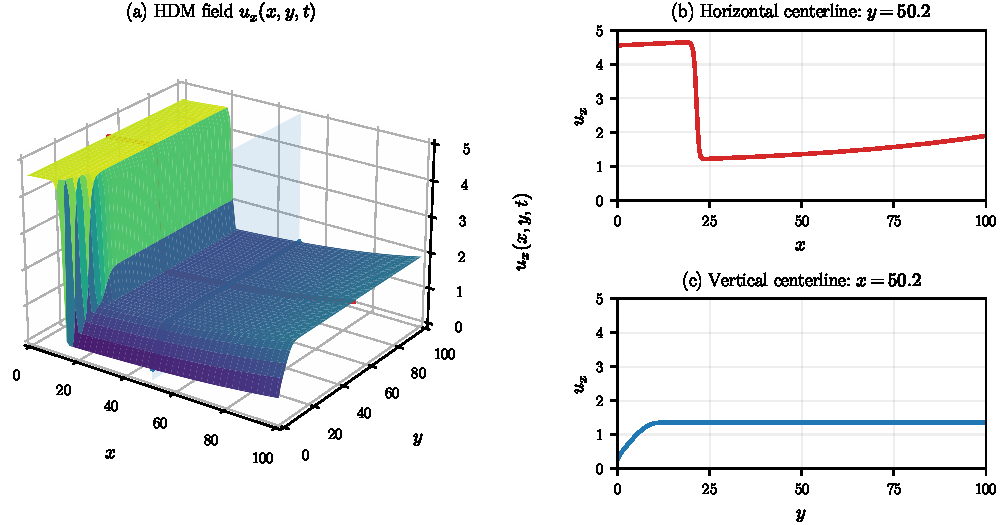
\includegraphics[width=0.96\linewidth]{figures/burgers_problem_3d.pdf}
 \caption{HDM solution at $\vect{\mu}=(4.56,0.019)$ and $t=7.5$: $u_x$ over the computational domain and two centerline slices.}
 \label{fig:burgers}
\end{figure}

\subsection{Reduced-order models and hyperreduction}

The common affine trial space is constructed from HDM solution trajectories computed on the nine-point parameter grid
\begin{equation}
 \{4.25,4.875,5.50\}\times\{0.015,0.0225,0.030\}.
\end{equation}
Each trajectory contributes 501 states, including its initial state, yielding $N_s=4\,509$ solution snapshots. Their mean defines the reference state $\vect{u}_{\mathrm{ref}}$. Applying the POD construction of Section~\ref{sec:prom} to the centered snapshots gives a ROB with $n=96$ modes, accounting for $99.950267\%$ of the sum of squared singular values. This ROB and reference state are used by both HPROMs.

To train the cubature rules, $N_c=225$ state pairs are selected, with 25 pairs distributed over the simulation interval at each training parameter. Each pair contains states at consecutive time levels, as required by the implicit time discretization. Both states are projected onto the affine trial space using Equation~\eqref{eq:projection}, and the associated local residuals and test-basis blocks provide the projected entity contributions used in the fits.

Stacking these contributions as in Equation~\eqref{eq:training-matrix} gives the classical training matrix with $21\,600$ rows and $62\,500$ columns. For BM-ECSW, the same entries are rearranged into 96 modal matrices of size $225\times62\,500$, following Equation~\eqref{eq:modal-matrix}. Both sampling procedures use the relative training tolerance $\tau=10^{-5}$. Their mesh sizes are determined by the selection and NNLS refitting needed to attain this tolerance, with no prescribed limit on the number of cells.

Table~\ref{tab:rules} reports the resulting reduced dimension $n$, sampled-mesh size $n_e$, augmented-mesh size $n_e^+$, relative fitting error $\eta$, and estimated offline training time. The timings are obtained from one fresh run per method on 20 CPU threads and include assembly of the training matrix, mesh sampling, and weight fitting. The common costs of generating HDM trajectories and constructing the POD basis are excluded.

\begin{table}[H]
 \centering\small
 \caption{Reduced-mesh sizes and estimated offline training times for the 2D parametric inviscid Burgers problem. Both rules use the same ROB, 225 state pairs, and relative training tolerance $\tau=10^{-5}$. Times correspond to one fresh training run per method on 20 CPU threads. The augmented size $n_e^+$ includes stencil support.}
 \label{tab:rules}
 \begin{tabular}{@{}lrrrrr@{}}
\toprule
Computational model & $n$ & $n_e$ & $n_e^+$ & $\eta$ & \shortstack{Offline training\\time (min)}\\
\midrule
HPROM (ECSW) & 96 & 2\,492 & 5\,914 & $9.795\times10^{-6}$ & 112.56\\
HPROM (BM-ECSW) & 96 & 300 & 868 & $8.359\times10^{-6}$ & 4.10\\
\bottomrule
\end{tabular}

\end{table}

Both rules attain the prescribed training tolerance. BM-ECSW selects 300 weighted cells, compared with $2\,492$ for classical ECSW, reducing the sampled-mesh size by a factor of $8.31$. The corresponding augmented meshes contain 868 and $5\,914$ cells. Because each cell carries two velocity unknowns, HPROM (BM-ECSW) reconstructs $1\,736$ state entries and evaluates 600 residual entries during time stepping, while HPROM (ECSW) reconstructs $11\,828$ state entries and evaluates $4\,984$ residual entries. The two models retain the same 96 generalized coordinates, so this reduction occurs in the local evaluations used to assemble their reduced equations.

The smaller BM mesh is accompanied by a larger set of scalar weights: $21\,597$ positive modal coefficients, compared with $2\,492$ weights for the classical rule. These coefficients multiply projected contributions formed from the evaluated local residual and test-basis blocks. Thus the number of stored and applied weights increases, while the number of cells required for the local evaluations decreases. Figure~\ref{fig:meshes} shows the sampled meshes together with the additional cells required by their residual stencils.

\begin{figure}[H]
 \centering
 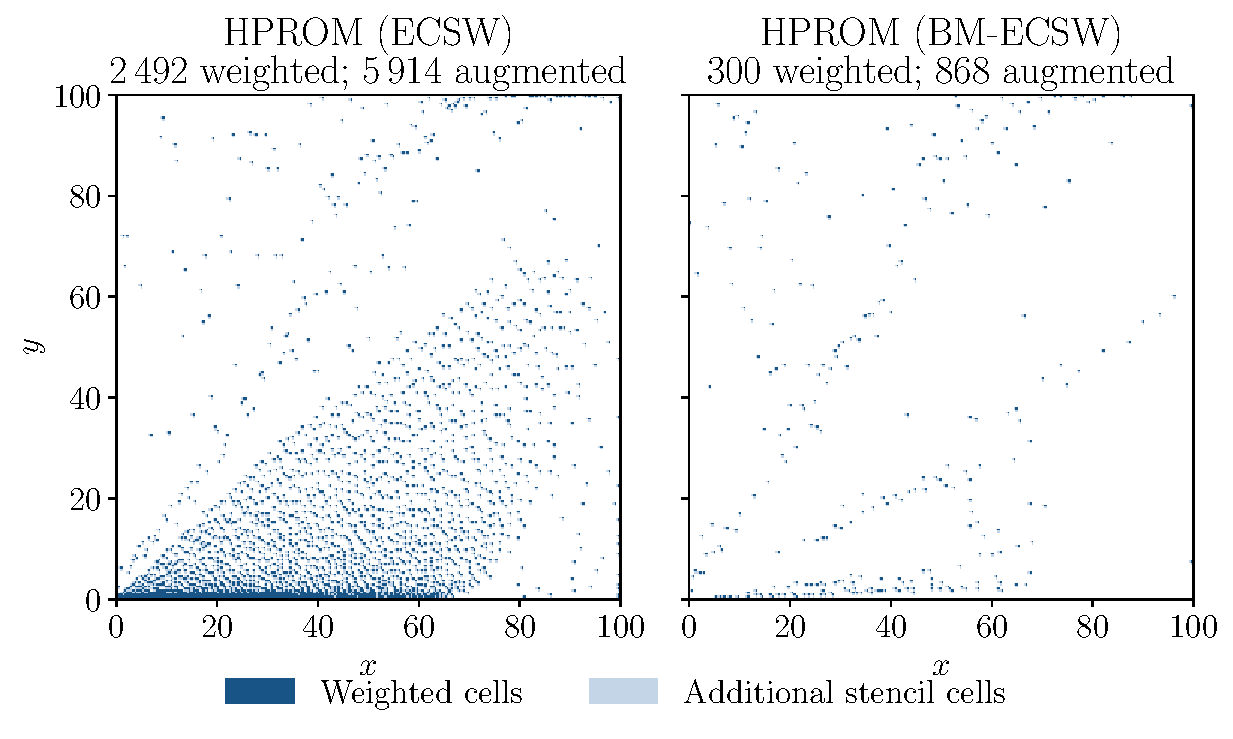
\includegraphics[width=0.88\linewidth]{figures/paper_sampled_cells.pdf}
 \caption{Reduced meshes for HPROM (ECSW) and HPROM (BM-ECSW). Dark blue marks weighted cells; light blue marks additional cells needed by the residual stencil.}
 \label{fig:meshes}
\end{figure}

The BM training procedure also has a lower measured offline cost in this comparison. Classical ECSW requires \ECSWOfflineMinutes{} minutes, whereas BM-ECSW requires \BMOfflineMinutes{} minutes, a reduction by a factor of \OfflineTrainingRatio{}.

\subsection{Accuracy and online performance}

The resulting HPROMs are evaluated at $\vect{\mu}=(4.56,0.019)$, $(4.75,0.020)$, and $(5.19,0.026)$. These parameter points lie inside $\mathcal D$ and are absent from the nine-point training grid. The HDM supplies the reference solution and serves as the full-order model (FOM) for the timing comparisons.

For these computations, both HPROMs use the previous reduced state as the initial guess at each time step and allow at most 20 nonlinear iterations. HPROM (ECSW) monitors the weighted sampled HDM residual norm, while HPROM (BM-ECSW) monitors the norm of its projected equations. Each solve uses a relative norm tolerance of $10^{-5}$ and a relative change threshold of $10^{-2}$ to detect a plateau. The classical solve applies full coordinate corrections; BM uses step control based on the decrease of its projected residual. These settings govern the online nonlinear solves and are separate from the cubature training tolerance.

Accuracy is measured over the complete solution trajectory using the global Euclidean relative error~\cite{ares2026closure}
\begin{equation}
 \mathbb{RE}_{2,\vect{u}}(\vect{\mu})
 =\left(\frac{\sum_{m=0}^{N_t}
              \|\vect{u}_{\mathrm{HDM}}^m(\vect{\mu})
                -\widetilde{\vect{u}}_{\mathrm{HPROM}}^m(\vect{\mu})\|_2^2}
             {\sum_{m=0}^{N_t}\|\vect{u}_{\mathrm{HDM}}^m(\vect{\mu})\|_2^2}
        \right)^{1/2},\qquad N_t=500.
 \label{eq:error}
\end{equation}
This measure includes both velocity components at all 501 states and is reported in percent. It accounts for the combined effects of the trial-space approximation, hyperreduction, and online solution procedure, whereas $\eta$ measures the offline fit of the projected training contributions. For the comparison over all queried parameters, the maximum trajectory error is defined as
\begin{equation}
 \mathbb{RE}_{2,\vect{u}}^{\max}
 =\max_{\vect{\mu}\in\mathcal D_{\mathrm{test}}}
             \mathbb{RE}_{2,\vect{u}}(\vect{\mu}),
 \qquad
 \mathcal D_{\mathrm{test}}=\{(4.56,0.019),(4.75,0.020),(5.19,0.026)\}.
 \label{eq:max-error}
\end{equation}

All computations are performed in double-precision arithmetic on an Intel Core Ultra 7 265 processor with 20 CPU threads. Each HPROM is run three times at each test parameter, and one FOM run per parameter supplies the reference time. The runs are executed sequentially, and the FOM nonlinear solver uses a relative residual tolerance of $10^{-12}$. Online times include solver setup and all 500 time steps; offline training, error assessment, and postprocessing are excluded. The mean HPROM time at each parameter is computed from its three repetitions, and the corresponding speedup factor is the FOM time divided by this mean. Wall-clock times in the main tables are reported in minutes.

\begin{table}[H]
 \centering\footnotesize
 \setlength{\tabcolsep}{3pt}
 \caption{Online performance comparison (accuracy and speedups relative to the FOM) for the 2D parametric inviscid Burgers problem at three unsampled parameter points. FOM: one run per parameter; HPROMs: mean of three runs, all on 20 CPU threads.}
 \label{tab:performance}
 \begin{tabular}{@{}lrrrrrrr@{}}
\toprule
Parameter & \multicolumn{2}{c}{Global Euclidean error (\%)} & \multicolumn{3}{c}{Wall-clock time (min)} & \multicolumn{2}{c}{Speedup factor}\\
\cmidrule(lr){2-3}\cmidrule(lr){4-6}\cmidrule(lr){7-8}
$(\mu_1,\mu_2)$ & \shortstack{HPROM\\(ECSW)} & \shortstack{HPROM\\(BM-ECSW)} & FOM & \shortstack{HPROM\\(ECSW)} & \shortstack{HPROM\\(BM-ECSW)} & \shortstack{HPROM\\(ECSW)} & \shortstack{HPROM\\(BM-ECSW)}\\
\midrule
$(4.56,0.019)$ & 1.0959 & 1.1019 & 5.387 & 0.30905 & 0.02031 & 17.43 & 265.25\\
$(4.75,0.020)$ & 1.0011 & 1.0061 & 5.388 & 0.31378 & 0.02007 & 17.17 & 268.52\\
$(5.19,0.026)$ & 0.9928 & 1.0069 & 5.438 & 0.30950 & 0.02014 & 17.57 & 270.05\\
\bottomrule
\end{tabular}

\end{table}

As shown in Table~\ref{tab:performance}, both HPROMs yield global errors close to $1\%$ at the three unsampled parameter points. Their maximum errors are \ECSWMaxGlobalError{}\% for HPROM (ECSW) and \BMMaxGlobalError{}\% for HPROM (BM-ECSW), and the largest error increase for the BM model relative to the classical model at an individual parameter is \BMLargestErrorIncrease{} percentage points. Every BM trajectory completes all 500 steps with the projected-equation tolerance satisfied within the iteration budget. Using the smaller BM mesh therefore retains comparable trajectory accuracy for this set of queried parameters.

Figure~\ref{fig:slices} compares horizontal centerline profiles at $\vect{\mu}=(4.56,0.019)$. Both HPROMs track the moving shock and closely follow the HDM profiles at the displayed times, with small oscillations near the discontinuity. These profiles illustrate the similar solution accuracy obtained with the two sampled meshes.

\begin{figure}[H]
 \centering
 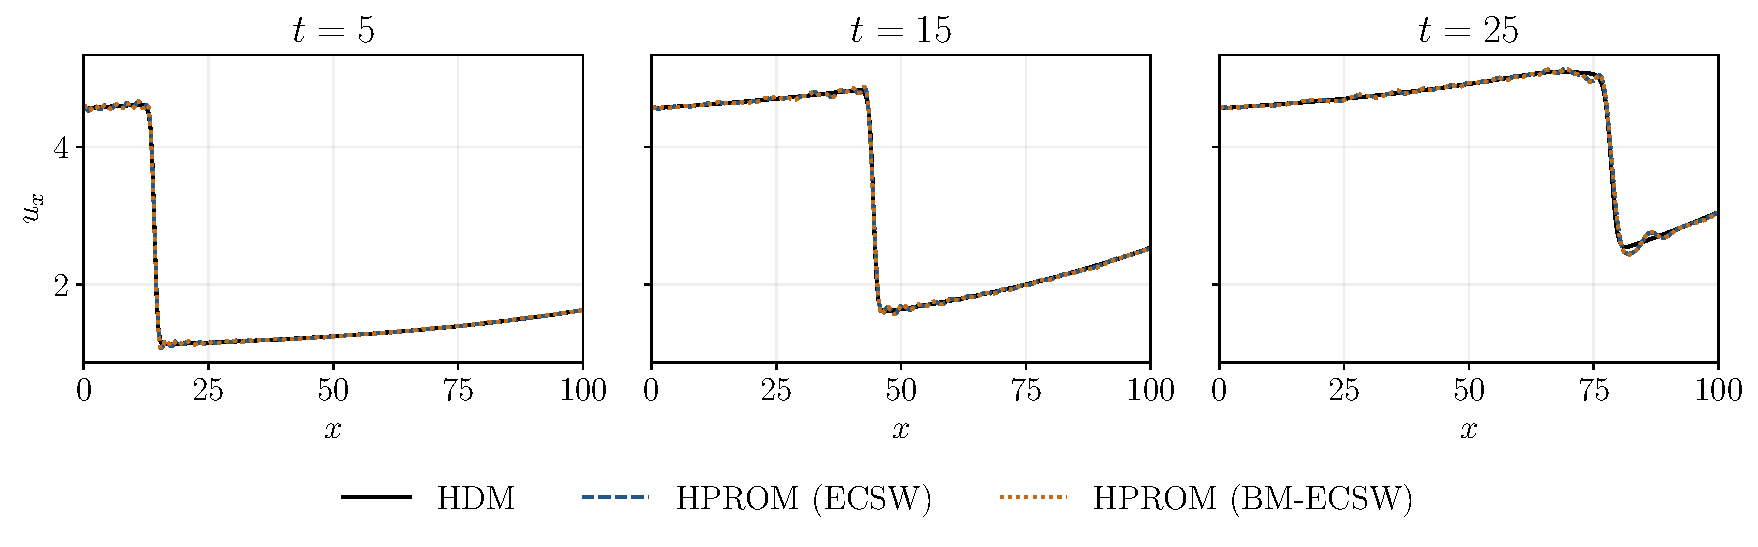
\includegraphics[width=\linewidth]{figures/paper_solution_slices.pdf}
 \caption{Horizontal centerline slices of $u_x$ at $y=50.2$, $\vect{\mu}=(4.56,0.019)$, and $t=5,15,25$. The three curves compare the HDM reference with HPROM (ECSW) and HPROM (BM-ECSW).}
 \label{fig:slices}
\end{figure}

To summarize the online cost over the three parameters, the HPROM times are averaged over all nine runs, and the FOM time is averaged over its three runs. Table~\ref{tab:summary} reports these mean times, the maximum errors in Equation~\eqref{eq:max-error}, and the speedup factors obtained by dividing the mean FOM time by the respective mean HPROM time.

\begin{table}[H]
 \centering\footnotesize
 \setlength{\tabcolsep}{4pt}
 \caption{Online performance summary for the 2D parametric inviscid Burgers problem: maximum global error, mean wall-clock time, and speedup relative to the FOM over the three unsampled parameter points.}
 \label{tab:summary}
 \begin{tabular}{@{}lrrrrrr@{}}
\toprule
Computational model & \shortstack{$n$\\($N$ for FOM)} & \shortstack{$n_e$\\($N_e$ for FOM)} & $n_e^+$ & $\mathbb{RE}_{2,\vect{u}}^{\max}$ (\%) & \shortstack{Wall-clock time\\(min)} & \shortstack{Speedup\\factor}\\
\midrule
FOM & 125\,000 & 62\,500 & 62\,500 & -- & 5.404 & --\\
HPROM (ECSW) & 96 & 2\,492 & 5\,914 & 1.0959 & 0.31078 & 17.39\\
HPROM (BM-ECSW) & 96 & 300 & 868 & 1.1019 & 0.02017 & 267.93\\
\bottomrule
\end{tabular}

\end{table}

The speedup factors based on the mean online times are \ECSWFOMSpeedup{} for HPROM (ECSW) and \BMFOMSpeedup{} for HPROM (BM-ECSW), relative to the FOM. Figure~\ref{fig:timings} shows the individual HPROM measurements and their spread around the means; the individual times and sample standard deviations are reported in Appendix~\ref{sec:repeated-measurements}.

\begin{figure}[H]
 \centering
 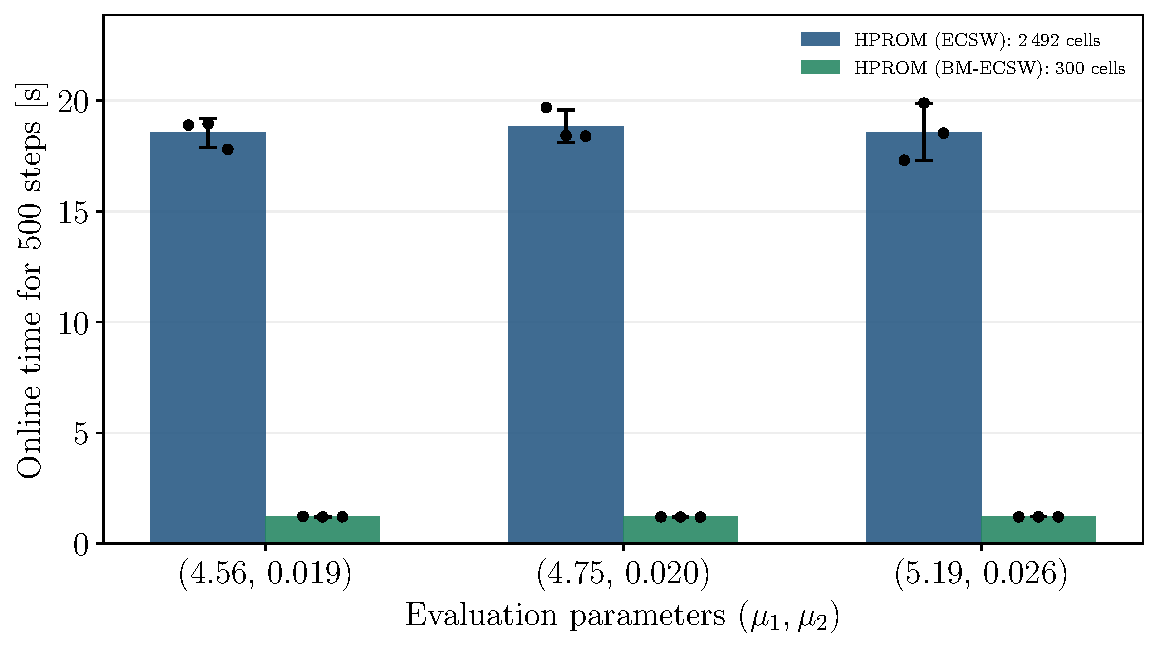
\includegraphics[width=0.88\linewidth]{figures/online_timings.pdf}
 \caption{Online times over three repetitions. Bars represent means, black points represent individual runs, and error bars represent sample standard deviations.}
 \label{fig:timings}
\end{figure}

The lower online cost of HPROM (BM-ECSW) is consistent with its smaller sampled and augmented meshes, which reduce the number of local residual and test-basis blocks evaluated during the nonlinear iterations. Both models use corrections assembled from linearized local residuals, but the measured solvers differ in their monitored norm and step control. The reported speedups therefore compare the complete online procedures at the stated accuracy. The single FOM run at each parameter supplies a reference time without estimating FOM timing variability.

\section{Current assessment}

BM-ECSW uses a shared reduced mesh and separate nonnegative modal fits against the full projected training targets. Its online Gauss--Newton-type update is assembled from local residuals and test-basis blocks on that mesh. The generalized coordinates are computed together.

For the two-dimensional parametric inviscid Burgers problem, the same 96-mode ROB, 225 training pairs, and $10^{-5}$ contribution-fit tolerance produce reduced meshes of 2\,492 cells for classical ECSW and 300 cells for BM. At three unsampled parameter points, the global errors remain close to $1\%$. The measured mean-time speedup factors relative to the FOM are \ECSWFOMSpeedup{} for HPROM (ECSW) and \BMFOMSpeedup{} for HPROM (BM-ECSW).

Mode-dependent weights enlarge the set of cubature fits available on a selected mesh. They also remove the automatic interpretation of the projected equations as derivatives of one sampled LSPG objective. The present results establish trajectory accuracy and online cost for the stated Burgers configuration. Training coverage and behavior outside the sampled parameter range remain to be assessed.

\appendix
\clearpage
\section{Common objectives, symmetry, and energy under modal weighting}
\label{sec:modal-structure}

Using different weights for the reduced components of one entity can change the gradient structure preserved by classical ECSW. The selected mesh and weights are fixed throughout this appendix, and the residuals and element potentials are assumed to be twice continuously differentiable.

\subsection{A common sampled least-squares objective}
\label{sec:appendix-common-objective}

\textit{Motivation:} LSPG obtains its projected equations by differentiating a scalar residual objective. We examine whether approximating those equations with classical ECSW and BM-ECSW preserves their interpretation as stationarity conditions of one scalar measure of error. The sampled entities and weights remain fixed throughout.

\subsubsection{LSPG stationarity equations}
\label{sec:appendix-lspg-foundations}

LSPG determines the reduced coordinates by minimizing the squared norm of the assembled HDM residual evaluated at the reconstructed state. The blocks $\vect{r}_e$ partition the residual rows, so the objective is the sum of their local scalar contributions $\phi_e$:
\begin{equation}
 \Phi(\vect{q})
 =\frac12\|\vect{r}(\vect{q})\|_2^2
 =\sum_{e\in\mathcal E}
   \underbrace{\frac12\vect{r}_e^T\vect{r}_e}_{\displaystyle\phi_e(\vect{q})}.
 \label{eq:appendix-objective-partition}
\end{equation}
To obtain the stationarity equations, differentiate each local contribution with respect to $\vect{q}$. With $\matr{W}_e=\partial\vect{r}_e/\partial\vect{q}$, the product rule gives
\begin{equation}
 \nabla_{\vect{q}}\phi_e
 =\frac12\left[\matr{W}_e^T\vect{r}_e
                   +(\vect{r}_e^T\matr{W}_e)^T\right]
 =\matr{W}_e^T\vect{r}_e.
 \label{eq:appendix-local-objective}
\end{equation}
The two terms in brackets are equal and cancel the factor $1/2$. Summing these local gradients gives the gradient of the complete objective:
\begin{equation}
 \nabla_{\vect{q}}\Phi
 =\sum_{e\in\mathcal E}\nabla_{\vect{q}}\phi_e
 =\sum_{e\in\mathcal E}\matr{W}_e^T\vect{r}_e
 =\vect{r}_n.
 \label{eq:appendix-full-gradient}
\end{equation}
This calculation produces the projected residual $\vect{r}_n$: setting it to zero imposes stationarity of $\Phi$. Stationarity is a necessary condition for an unconstrained minimum, and alone does not establish a minimum.

\subsubsection{Classical ECSW}
\label{sec:appendix-classical-objective}

Classical ECSW approximates these stationarity equations by replacing the full sum with a weighted sum over the sampled entities:
\begin{equation}
 \widetilde{\vect{r}}_n^{\mathrm{ECSW}}
 =\sum_{e\in\widetilde{\mathcal E}}\xi_e\matr{W}_e^T\vect{r}_e.
 \label{eq:appendix-classical-projected-vector}
\end{equation}
To check whether this approximation is still a gradient, consider the corresponding weighted least-squares objective:
\begin{equation}
 \Phi_{\mathrm{ECSW}}(\vect{q})
 =\frac12\sum_{e\in\widetilde{\mathcal E}}\xi_e\|\vect{r}_e(\vect{q})\|_2^2
 =\sum_{e\in\widetilde{\mathcal E}}\xi_e\phi_e.
 \label{eq:appendix-classical-objective}
\end{equation}
The weights are fixed scalars, so differentiation gives
\begin{equation}
 \nabla_{\vect{q}}\Phi_{\mathrm{ECSW}}
 =\sum_{e\in\widetilde{\mathcal E}}\xi_e\nabla_{\vect{q}}\phi_e
 =\sum_{e\in\widetilde{\mathcal E}}\xi_e\matr{W}_e^T\vect{r}_e
 =\widetilde{\vect{r}}_n^{\mathrm{ECSW}}.
 \label{eq:appendix-classical-gradient}
\end{equation}
Thus the approximation preserves the gradient relation. Solving $\widetilde{\vect{r}}_n^{\mathrm{ECSW}}=\vect{0}$ imposes stationarity of $\Phi_{\mathrm{ECSW}}$. This sampled objective generally differs from $\Phi$, but all reduced equations are derivatives of this same scalar function. Different entities can have different weights; each entity's weight is shared by every component of its contribution.

\subsubsection{BM-ECSW}
\label{sec:appendix-bm-objective}

BM-ECSW instead assigns a separate weight to each reduced component:
\begin{equation}
 \widetilde{\vect{r}}_n^{\mathrm{BM}}
 =\sum_{e\in\widetilde{\mathcal E}}\matr{D}_e\matr{W}_e^T\vect{r}_e,
 \qquad\matr{D}_e=\operatorname{diag}(\xi_{e,1},\ldots,\xi_{e,n}).
 \label{eq:appendix-bm-projected-vector}
\end{equation}
We ask the same question: is this vector the gradient of a common scalar objective? If a smooth function $\Phi_{\mathrm{BM}}$ generates it, its components are $\widetilde r_{n,i}^{\mathrm{BM}}=\partial\Phi_{\mathrm{BM}}/\partial q_i$. Continuity of the second derivatives then requires
\begin{equation}
 \frac{\partial\widetilde r_{n,i}^{\mathrm{BM}}}{\partial q_j}
 =\frac{\partial^2\Phi_{\mathrm{BM}}}{\partial q_j\partial q_i}
 =\frac{\partial^2\Phi_{\mathrm{BM}}}{\partial q_i\partial q_j}
 =\frac{\partial\widetilde r_{n,j}^{\mathrm{BM}}}{\partial q_i},
 \qquad i,j=1,\ldots,n.
 \label{eq:appendix-common-potential-test}
\end{equation}
This condition tests the BM vector directly, without selecting a candidate objective. Unequal crossed derivatives at a point exclude every smooth scalar function whose gradient could equal that vector in a neighborhood of the point.

Component $i$ of the BM vector can be written as
\begin{equation}
 \widetilde r_{n,i}^{\mathrm{BM}}
 =\sum_{e\in\widetilde{\mathcal E}}\xi_{e,i}
                       \matr{W}_e(:,i)^T\vect{r}_e
 =\sum_{e\in\widetilde{\mathcal E}}\xi_{e,i}
                         \frac{\partial\phi_e}{\partial q_i}.
 \label{eq:appendix-bm-weighted-gradients}
\end{equation}
The second equality uses component $i$ of the local gradient identity in Equation~\eqref{eq:appendix-local-objective}.
The fixed weights remain outside the derivatives. Differentiating components $i$ and $j$ gives
\begin{equation}
 \begin{aligned}
 \frac{\partial\widetilde r_{n,i}^{\mathrm{BM}}}{\partial q_j}
 &=\sum_{e\in\widetilde{\mathcal E}}\xi_{e,i}
                  \frac{\partial^2\phi_e}{\partial q_j\partial q_i},\\
 \frac{\partial\widetilde r_{n,j}^{\mathrm{BM}}}{\partial q_i}
 &=\sum_{e\in\widetilde{\mathcal E}}\xi_{e,j}
                  \frac{\partial^2\phi_e}{\partial q_i\partial q_j}.
 \end{aligned}
 \label{eq:appendix-bm-cross-derivatives}
\end{equation}
The local mixed derivatives agree, but the weights multiplying them can differ. Subtracting yields
\begin{equation}
 \frac{\partial\widetilde r_{n,i}^{\mathrm{BM}}}{\partial q_j}
 -\frac{\partial\widetilde r_{n,j}^{\mathrm{BM}}}{\partial q_i}
 =\sum_{e\in\widetilde{\mathcal E}}(\xi_{e,i}-\xi_{e,j})
                  \frac{\partial^2\phi_e}{\partial q_i\partial q_j}.
 \label{eq:appendix-modal-compatibility}
\end{equation}
Classical ECSW makes each term zero because $\xi_{e,i}=\xi_{e,j}=\xi_e$. BM-ECSW does not enforce this equality. Different weights can still give a zero sum through zero local mixed derivatives or cancellation, but positivity alone does not ensure it. If the sum is nonzero, the BM vector cannot be the gradient of a common scalar objective near that point. The following example demonstrates this loss of gradient structure.

\subsubsection{Numerical example}
\label{sec:appendix-lspg-numerical-example}

Consider three scalar residual blocks depending on two reduced coordinates:
\begin{equation}
 \vect{r}(\vect{q})
 =\begin{pmatrix}r_1\\r_2\\r_3\end{pmatrix}
 =\begin{pmatrix}q_1\\q_2\\q_1+q_2^2-3\end{pmatrix}.
 \label{eq:appendix-example-residuals}
\end{equation}
Each residual block is scalar, so its test-basis row is
\[
 \matr{W}_1=(1,0),\qquad
 \matr{W}_2=(0,1),\qquad
 \matr{W}_3=(1,2q_2).
\]
We construct both projected vectors from these same residuals and test-basis rows, then check whether each vector is a gradient. Both rules use all three entities; only the weight of entity 3 in the second equation changes. In $\matr{\Xi}$, rows identify entities and columns identify reduced equations.

\begin{subequations}
 \label{eq:appendix-example-weights}
 \noindent
 \begin{minipage}[t]{0.48\linewidth}
  \vspace{0pt}\raggedright
  \textbf{Classical ECSW}\par\smallskip
  \small
  The entity weights are
  \begin{equation}
   \begin{gathered}
    \vect{\xi}=\begin{pmatrix}2\\3\\2\end{pmatrix}.
   \end{gathered}
  \end{equation}
 \end{minipage}\hfill
 \begin{minipage}[t]{0.48\linewidth}
  \vspace{0pt}\raggedright
  \textbf{BM-ECSW}\par\smallskip
  \small
  The modal weights are
  \begin{equation}
   \begin{gathered}
    \matr{\Xi}=\begin{pmatrix}2&2\\3&3\\2&1\end{pmatrix}.
   \end{gathered}
  \end{equation}
 \end{minipage}
\end{subequations}

\begin{subequations}
 \label{eq:appendix-example-projected-vectors}
 \noindent
 \begin{minipage}[t]{0.48\linewidth}
  \vspace{0pt}\small\raggedright
  The classical rule defines the projected vector
  \begin{equation}
   \widetilde{\vect{r}}_n^{\mathrm{ECSW}}
   =\sum_{e=1}^{3}\xi_e\matr{W}_e^T r_e.
  \end{equation}
 \end{minipage}\hfill
 \begin{minipage}[t]{0.48\linewidth}
  \vspace{0pt}\small\raggedright
  The BM rule defines the projected vector
  \begin{equation}
   \widetilde{\vect{r}}_n^{\mathrm{BM}}
   =\sum_{e=1}^{3}\matr{D}_e\matr{W}_e^T r_e.
  \end{equation}
 \end{minipage}
\end{subequations}

Using the residuals and test-basis rows above gives the projected components for both rules.

\begin{subequations}
 \label{eq:appendix-example-bm}
 \noindent
 \begin{minipage}[t]{0.48\linewidth}
  \vspace{0pt}\small\raggedright
  Assembling the weighted contributions gives
  \begin{equation}
   \begin{aligned}
    \widetilde r_{n,1}^{\mathrm{ECSW}}
     &=2r_1+2r_3\\
     &=2q_1+2r_3,\\
    \widetilde r_{n,2}^{\mathrm{ECSW}}
     &=3r_2+4q_2r_3\\
     &=3q_2+4q_2r_3.
   \end{aligned}
  \end{equation}
 \end{minipage}\hfill
 \begin{minipage}[t]{0.48\linewidth}
  \vspace{0pt}\small\raggedright
  Assembling the weighted contributions gives
  \begin{equation}
   \begin{aligned}
    \widetilde r_{n,1}^{\mathrm{BM}}
     &=2r_1+2r_3\\
     &=2q_1+2r_3,\\
    \widetilde r_{n,2}^{\mathrm{BM}}
     &=3r_2+2q_2r_3\\
     &=3q_2+2q_2r_3.
   \end{aligned}
  \end{equation}
 \end{minipage}
\end{subequations}

We now differentiate the first component with respect to $q_2$ and the second with respect to $q_1$, as required by Equation~\eqref{eq:appendix-common-potential-test}.

\begin{subequations}
 \label{eq:appendix-example-cross-partials}
 \noindent
 \begin{minipage}[t]{0.48\linewidth}
  \vspace{0pt}\small\raggedright
  The mixed derivatives are
  \begin{equation}
   \begin{aligned}
    \frac{\partial\widetilde r_{n,1}^{\mathrm{ECSW}}}{\partial q_2}
     &=2\frac{\partial r_3}{\partial q_2}=4q_2,\\
    \frac{\partial\widetilde r_{n,2}^{\mathrm{ECSW}}}{\partial q_1}
     &=4q_2\frac{\partial r_3}{\partial q_1}=4q_2.
   \end{aligned}
  \end{equation}
 \end{minipage}\hfill
 \begin{minipage}[t]{0.48\linewidth}
  \vspace{0pt}\small\raggedright
  The mixed derivatives are
  \begin{equation}
   \begin{aligned}
    \frac{\partial\widetilde r_{n,1}^{\mathrm{BM}}}{\partial q_2}
     &=2\frac{\partial r_3}{\partial q_2}=4q_2,\\
    \frac{\partial\widetilde r_{n,2}^{\mathrm{BM}}}{\partial q_1}
     &=2q_2\frac{\partial r_3}{\partial q_1}=2q_2.
   \end{aligned}
  \end{equation}
 \end{minipage}
\end{subequations}


\noindent
\begin{minipage}[t]{0.48\linewidth}
 \vspace{0pt}\small\raggedright
 The crossed derivatives agree for all $\vect{q}$. The common scalar objective is
 \[
  \Phi_{\mathrm{ECSW}}
  =\frac12\left(2q_1^2+3q_2^2+2r_3^2\right).
 \]
 Its gradient reproduces both classical components in Equation~\eqref{eq:appendix-example-bm}.
\end{minipage}\hfill
\begin{minipage}[t]{0.48\linewidth}
 \vspace{0pt}\small\raggedright
 The crossed derivatives differ by $2q_2$, violating Equation~\eqref{eq:appendix-common-potential-test} whenever $q_2\ne0$. Entities 1 and 2 contribute zero to this difference; entity 3 contributes $2q_2$. Hence no smooth scalar function has this BM vector as its gradient near such a point.
\end{minipage}

Both rules select every entity with positive weights. Changing the weight of entity 3 in the second BM component from 1 to 2 recovers the classical vector and its common objective.

The example establishes what modal weighting can change. BM still approximates the full projected residual $\vect{r}_n=\nabla_{\vect{q}}\Phi$, and its online problem remains $\widetilde{\vect{r}}_n^{\mathrm{BM}}=\vect{0}$. However, the approximation need not itself be a gradient. When the difference in Equation~\eqref{eq:appendix-modal-compatibility} is nonzero, its equations cannot be interpreted directly as the stationarity conditions of one common sampled least-squares objective.

This conclusion does not imply that the BM equations have no solution or that the online iteration must fail. It identifies the gradient structure that is no longer guaranteed, so the classical objective-based descent argument cannot be assumed for BM. Section~\ref{sec:appendix-update-structure} examines this consequence for the online correction. Preserving a common gradient would require the equality in Equation~\eqref{eq:appendix-common-potential-test} throughout the coordinate domain; the projected-residual training tolerance does not impose that condition.

\subsection{Symmetry and the online correction}
\label{sec:appendix-update-structure}

The classical Gauss--Newton matrix is a sum of weighted Gram matrices,
\begin{equation}
 \widehat{\matr{J}}_n^{\mathrm{ECSW}}
 =\sum_{e\in\widetilde{\mathcal E}}\xi_e\matr{W}_e^T\matr{W}_e,
 \qquad
 \vect{z}^T\widehat{\matr{J}}_n^{\mathrm{ECSW}}\vect{z}
 =\sum_{e\in\widetilde{\mathcal E}}\xi_e\|\matr{W}_e\vect{z}\|_2^2\geq0.
 \label{eq:appendix-classical-gram}
\end{equation}
It is symmetric positive semidefinite, and positive definite if the blocks with positive weights have no common nonzero null direction. Under this rank condition, the correction in Equation~\eqref{eq:classical-gn} is a descent direction for $\Phi_{\mathrm{ECSW}}$ at a nonstationary point:
\begin{equation}
 \nabla\Phi_{\mathrm{ECSW}}^T\Delta\vect{q}
 =-\bigl(\widetilde{\vect{r}}_n^{\mathrm{ECSW}}\bigr)^T
       \bigl(\widehat{\matr{J}}_n^{\mathrm{ECSW}}\bigr)^{-1}
         \widetilde{\vect{r}}_n^{\mathrm{ECSW}}<0.
 \label{eq:appendix-classical-descent}
\end{equation}
Thus a sufficiently small positive step decreases the sampled objective; a full step need not do so.

In BM-ECSW, different rows of each local Gram matrix carry different weights. Subtracting its transposed entries gives
\begin{equation}
 \bigl(\widehat J_n^{\mathrm{BM}}\bigr)_{ij}
 -\bigl(\widehat J_n^{\mathrm{BM}}\bigr)_{ji}
 =\sum_{e\in\widetilde{\mathcal E}}
       (\xi_{e,i}-\xi_{e,j})\matr{W}_e(:,i)^T\matr{W}_e(:,j).
 \label{eq:appendix-bm-matrix-asymmetry}
\end{equation}
\textbf{Positive modal weights do not guarantee symmetry or the classical descent property.} The latter also requires the projected vector to be the gradient of the objective whose decrease is being considered.

The vanishing of the difference in Equation~\eqref{eq:appendix-modal-compatibility} tests the gradient structure of the nonlinear projected vector. Equation~\eqref{eq:appendix-bm-matrix-asymmetry} concerns the online update matrix, obtained by holding $\matr{W}_e$ fixed when linearizing the local residuals. These matrices coincide for affine residuals; otherwise, differentiating the projected vector also differentiates $\matr{W}_e$. Both online algorithms in the main text use only residuals and their first derivatives.

Loss of symmetry does not by itself imply a different correction or failure of the solve. For example, if $\matr{D}_e=\xi_e\matr{D}$ for a common positive diagonal matrix $\matr{D}$, then
\begin{equation}
 \widetilde{\vect{r}}_n^{\mathrm{BM}}
 =\matr{D}\widetilde{\vect{r}}_n^{\mathrm{ECSW}},
 \qquad
 \widehat{\matr{J}}_n^{\mathrm{BM}}
 =\matr{D}\widehat{\matr{J}}_n^{\mathrm{ECSW}}.
 \label{eq:appendix-shared-row-scaling}
\end{equation}
Multiplying by $\matr{D}^{-1}$ recovers the classical equations and correction system. Their roots and corrections are therefore identical, although the BM matrix may be nonsymmetric. Independent modal fitting does not impose this factorization.

\subsection{Potential energy in conservative structural dynamics}
\label{sec:appendix-mechanical-energy}

In conservative structural dynamics, the internal force derives from a mechanical potential~\cite{farhat2015structure}. With a constant symmetric positive definite mass matrix $\matr{M}$ and no external loading, the HDM satisfies
\begin{equation}
 \matr{M}\ddot{\vect{u}}+\nabla_{\vect{u}}\mathcal V^{\mathrm{int}}(\vect{u})
 =\vect{0},
 \qquad
 \mathcal V^{\mathrm{int}}(\vect{u})
 =\sum_{e\in\mathcal E}\mathcal V_e^{\mathrm{int}}(\matr{L}_e\vect{u}),
 \label{eq:appendix-hdm-potential}
\end{equation}
where $\matr{L}_e$ extracts the displacement entries of element $e$. The restoring force is $-\nabla_{\vect{u}}\mathcal V^{\mathrm{int}}$. Under $\vect{u}=\matr{V}\vect{q}$, define $\matr{M}_r=\matr{V}^T\matr{M}\matr{V}$ and
\[
 \mathcal V_{e,r}^{\mathrm{int}}(\vect{q})
 =\mathcal V_e^{\mathrm{int}}(\matr{L}_e\matr{V}\vect{q}).
\]
Classical ECSW weights these element potentials to obtain the sampled potential and its equations of motion:
\begin{equation}
 \widetilde{\mathcal V}_r^{\mathrm{int}}
 =\sum_{e\in\widetilde{\mathcal E}}\xi_e\mathcal V_{e,r}^{\mathrm{int}},
 \qquad
 \matr{M}_r\ddot{\vect{q}}
   +\nabla_{\vect{q}}\widetilde{\mathcal V}_r^{\mathrm{int}}=\vect{0}.
 \label{eq:appendix-ecsw-potential}
\end{equation}
Consequently, the sampled system has the mechanical energy
\begin{equation}
 \begin{aligned}
 \widetilde{\mathcal H}_r
 &=\frac12\dot{\vect{q}}^T\matr{M}_r\dot{\vect{q}}
       +\widetilde{\mathcal V}_r^{\mathrm{int}},\\
 \frac{d\widetilde{\mathcal H}_r}{dt}
 &=\dot{\vect{q}}^T
      \left(\matr{M}_r\ddot{\vect{q}}
               +\nabla_{\vect{q}}\widetilde{\mathcal V}_r^{\mathrm{int}}\right)
 =0.
 \end{aligned}
 \label{eq:appendix-ecsw-energy-balance}
\end{equation}
The sampled mechanical energy is therefore conserved in continuous time; conservation after time discretization depends on the integrator. \textbf{This mechanical potential is distinct from the LSPG least-squares objective.}

Modal weighting replaces the internal term by
\begin{equation}
 \widetilde{\vect{f}}_r^{\mathrm{int},\mathrm{BM}}
 =\sum_{e\in\widetilde{\mathcal E}}
       \matr{D}_e\nabla_{\vect{q}}\mathcal V_{e,r}^{\mathrm{int}},
 \qquad
 \matr{M}_r\ddot{\vect{q}}+\widetilde{\vect{f}}_r^{\mathrm{int},\mathrm{BM}}=\vect{0}.
 \label{eq:appendix-bm-structural-motion}
\end{equation}
A potential generating this internal term requires the right-hand side of Equation~\eqref{eq:appendix-modal-compatibility} to vanish, with $\phi_e$ replaced by $\mathcal V_{e,r}^{\mathrm{int}}$. If that condition fails, the energy construction in Equation~\eqref{eq:appendix-ecsw-energy-balance} no longer applies with the original reduced kinetic energy. This issue also arises in Galerkin structural models.

The effect on stiffness follows by defining $\matr{K}_{e,r}=\nabla_{\vect{q}}^2\mathcal V_{e,r}^{\mathrm{int}}$:
\begin{equation}
 \matr{K}_r^{\mathrm{ECSW}}
 =\sum_{e\in\widetilde{\mathcal E}}\xi_e\matr{K}_{e,r},
 \qquad
 \matr{K}_r^{\mathrm{BM}}
 =\sum_{e\in\widetilde{\mathcal E}}\matr{D}_e\matr{K}_{e,r}.
 \label{eq:appendix-structural-stiffness}
\end{equation}
Classical ECSW preserves symmetry of the element Hessians. If these Hessians are positive semidefinite, positive weights preserve that property; positive definiteness further requires that the selected Hessians have no common nonzero null direction. An SPD assembled HDM operator alone does not establish these conditions.

Even when these conditions hold, positive modal weights can change the stability of the structural system. Consider two reduced element potentials,
\begin{equation}
 \mathcal V_{1,r}^{\mathrm{int}}=\frac12(q_1+q_2)^2,
 \qquad
 \mathcal V_{2,r}^{\mathrm{int}}=\frac12(q_1+2q_2)^2,
 \label{eq:appendix-two-element-potentials}
\end{equation}
with positive semidefinite Hessians
\[
 \matr{K}_{1,r}=\begin{pmatrix}1&1\\1&1\end{pmatrix},
 \qquad
 \matr{K}_{2,r}=\begin{pmatrix}1&2\\2&4\end{pmatrix}.
\]
Classical weights $\xi_1=\xi_2=1$ give an SPD stiffness, whereas BM weights $\matr{D}_1=\operatorname{diag}(1,4)$ and $\matr{D}_2=\matr{I}_2$ give
\begin{equation}
 \matr{K}_r^{\mathrm{ECSW}}
 =\begin{pmatrix}2&3\\3&5\end{pmatrix},
 \qquad
 \matr{K}_r^{\mathrm{BM}}
 =\begin{pmatrix}2&3\\6&8\end{pmatrix}.
 \label{eq:appendix-negative-eigenvalue-example}
\end{equation}
The BM stiffness has determinant $-2$ and a negative eigenvalue $\lambda_-=5-3\sqrt3$. With $\matr{M}_r=\matr{I}_2$, motion along the associated eigenvector satisfies $\ddot a+\lambda_-a=0$ and admits exponential growth proportional to $\exp(\sqrt{-\lambda_-}\,t)$.

Both elements remain selected and every weight is positive: \textbf{positivity alone does not preserve stability in this structural example}. Training accuracy may exclude these particular weights, but does not explicitly impose potential compatibility or stiffness symmetry. The growing mode follows from the structural equation of motion; nonsymmetry alone does not establish failure of a BM LSPG online solve.


\clearpage
\section{Individual online measurements}
\label{sec:repeated-measurements}

Table~\ref{tab:timings} reports the individual online times in seconds. SD is the sample standard deviation, computed with denominator $3-1$.

\begin{table}[H]
 \centering\footnotesize
 \setlength{\tabcolsep}{4pt}
 \caption{Individual online wall-clock times (seconds) for HPROM (ECSW) and HPROM (BM-ECSW) at the three unsampled parameter points. Each measurement uses a fresh process and 20 CPU threads.}
 \label{tab:timings}
 \begin{tabular}{@{}llrrrrr@{}}
\toprule
Parameter & Computational model & Run 1 & Run 2 & Run 3 & Mean & SD\\
\midrule
$(4.56,0.019)$ & HPROM (ECSW) & 18.889 & 18.945 & 17.795 & 18.543 & 0.648\\
$(4.56,0.019)$ & HPROM (BM-ECSW) & 1.238 & 1.205 & 1.212 & 1.218 & 0.017\\
\addlinespace
$(4.75,0.020)$ & HPROM (ECSW) & 19.682 & 18.408 & 18.390 & 18.827 & 0.741\\
$(4.75,0.020)$ & HPROM (BM-ECSW) & 1.209 & 1.204 & 1.200 & 1.204 & 0.005\\
\addlinespace
$(5.19,0.026)$ & HPROM (ECSW) & 17.304 & 19.880 & 18.526 & 18.570 & 1.288\\
$(5.19,0.026)$ & HPROM (BM-ECSW) & 1.206 & 1.211 & 1.208 & 1.208 & 0.002\\
\addlinespace
\bottomrule
\end{tabular}

\end{table}

\begin{table}[H]
 \centering\small
 \caption{Fresh production FOM integration times: one run at each queried parameter, 20 CPU threads, and 500 time steps. The last row is the arithmetic mean over the three parameters.}
 \label{tab:fom-timings}
 \begin{tabular}{@{}lrr@{}}
\toprule
Parameter & Wall-clock time (s) & Wall-clock time (min)\\
\midrule
$(4.56,0.019)$ & 323.195 & 5.387\\
$(4.75,0.020)$ & 323.275 & 5.388\\
$(5.19,0.026)$ & 326.310 & 5.438\\
Mean & 324.260 & 5.404\\
\bottomrule
\end{tabular}

\end{table}

\begin{thebibliography}{99}
\bibitem{ares2026closure}
S.~Ares De Parga, R.~Tezaur, C.~G.~Hern\'andez, and C.~Farhat.
Nonlinear projection-based model order reduction with machine learning regression for closure error modeling in the latent space.
\textit{Computer Methods in Applied Mechanics and Engineering}, 448:118443, 2026.
DOI: \href{https://doi.org/10.1016/j.cma.2025.118443}{10.1016/j.cma.2025.118443}.

\bibitem{carlberg2011efficient}
K.~Carlberg, C.~Bou-Mosleh, and C.~Farhat.
Efficient non-linear model reduction via a least-squares Petrov--Galerkin projection and compressive tensor approximations.
\textit{International Journal for Numerical Methods in Engineering}, 86:155--181, 2011.

\bibitem{carlberg2013gnat}
K.~Carlberg, C.~Farhat, J.~Cortial, and D.~Amsallem.
The GNAT method for nonlinear model reduction: effective implementation and application to computational fluid dynamics and turbulent flows.
\textit{Journal of Computational Physics}, 242:623--647, 2013.
DOI: \href{https://doi.org/10.1016/j.jcp.2013.02.028}{10.1016/j.jcp.2013.02.028}.

\bibitem{farhat2014dimensional}
C.~Farhat, P.~Avery, T.~Chapman, and J.~Cortial.
Dimensional reduction of nonlinear finite element dynamic models with finite rotations and energy-based mesh sampling and weighting for computational efficiency.
\textit{International Journal for Numerical Methods in Engineering}, 98:625--662, 2014.
DOI: \href{https://doi.org/10.1002/nme.4668}{10.1002/nme.4668}.

\bibitem{farhat2015structure}
C.~Farhat, T.~Chapman, and P.~Avery.
Structure-preserving, stability, and accuracy properties of the energy-conserving sampling and weighting method for the hyper reduction of nonlinear finite element dynamic models.
\textit{International Journal for Numerical Methods in Engineering}, 102:1077--1110, 2015.
DOI: \href{https://doi.org/10.1002/nme.4820}{10.1002/nme.4820}.

\bibitem{chapman2017accelerated}
T.~Chapman, P.~Avery, P.~Collins, and C.~Farhat.
Accelerated mesh sampling for the hyper reduction of nonlinear computational models.
\textit{International Journal for Numerical Methods in Engineering}, 109(12):1623--1654, 2017.
DOI: \href{https://doi.org/10.1002/nme.5332}{10.1002/nme.5332}.

\bibitem{grimberg2021mesh}
S.~Grimberg, C.~Farhat, R.~Tezaur, and C.~Bou-Mosleh.
Mesh sampling and weighting for the hyperreduction of nonlinear Petrov--Galerkin reduced-order models with local reduced-order bases.
\textit{International Journal for Numerical Methods in Engineering}, 122:1846--1874, 2021.
DOI: \href{https://doi.org/10.1002/nme.6603}{10.1002/nme.6603}.

\bibitem{barnett2023neural}
J.~Barnett, C.~Farhat, and Y.~Maday.
Neural-network-augmented projection-based model order reduction for mitigating the Kolmogorov barrier to reducibility.
\textit{Journal of Computational Physics}, 492:112420, 2023.

\bibitem{rodriguez2026proposal}
S.~Rodriguez.
Proposal on ECSW.
Unpublished technical note, September 30, 2026.

\bibitem{tropp2006simultaneous}
J.~A.~Tropp, A.~C.~Gilbert, and M.~J.~Strauss.
Algorithms for simultaneous sparse approximation. Part I: Greedy pursuit.
\textit{Signal Processing}, 86(3):572--588, 2006.
DOI: \href{https://doi.org/10.1016/j.sigpro.2005.05.030}{10.1016/j.sigpro.2005.05.030}.

\end{thebibliography}
\end{document}
